% Options for packages loaded elsewhere
\PassOptionsToPackage{unicode}{hyperref}
\PassOptionsToPackage{hyphens}{url}
%
\documentclass[
]{article}
\usepackage{amsmath,amssymb}
\usepackage{lmodern}
\usepackage{ifxetex,ifluatex}
\ifnum 0\ifxetex 1\fi\ifluatex 1\fi=0 % if pdftex
  \usepackage[T1]{fontenc}
  \usepackage[utf8]{inputenc}
  \usepackage{textcomp} % provide euro and other symbols
\else % if luatex or xetex
  \usepackage{unicode-math}
  \defaultfontfeatures{Scale=MatchLowercase}
  \defaultfontfeatures[\rmfamily]{Ligatures=TeX,Scale=1}
\fi
% Use upquote if available, for straight quotes in verbatim environments
\IfFileExists{upquote.sty}{\usepackage{upquote}}{}
\IfFileExists{microtype.sty}{% use microtype if available
  \usepackage[]{microtype}
  \UseMicrotypeSet[protrusion]{basicmath} % disable protrusion for tt fonts
}{}
\makeatletter
\@ifundefined{KOMAClassName}{% if non-KOMA class
  \IfFileExists{parskip.sty}{%
    \usepackage{parskip}
  }{% else
    \setlength{\parindent}{0pt}
    \setlength{\parskip}{6pt plus 2pt minus 1pt}}
}{% if KOMA class
  \KOMAoptions{parskip=half}}
\makeatother
\usepackage{xcolor}
\IfFileExists{xurl.sty}{\usepackage{xurl}}{} % add URL line breaks if available
\IfFileExists{bookmark.sty}{\usepackage{bookmark}}{\usepackage{hyperref}}
\hypersetup{
  pdftitle={A Tutorial on Time-Dependent Cohort State-Transition Models in R},
  pdfauthor={Fernando Alarid-Escudero, PhD; Eline Krijkamp, MSc; Eva A. Enns, PhD; Alan Yang, MSc; Myriam G.M. Hunink, PhD\^{}\textbackslash dagger; Petros Pechlivanoglou, PhD; Hawre Jalal, MD, PhD},
  pdfkeywords={Markov models, state-transition models, decision models, Tutorial, R},
  hidelinks,
  pdfcreator={LaTeX via pandoc}}
\urlstyle{same} % disable monospaced font for URLs
\usepackage[margin=1in]{geometry}
\usepackage{color}
\usepackage{fancyvrb}
\newcommand{\VerbBar}{|}
\newcommand{\VERB}{\Verb[commandchars=\\\{\}]}
\DefineVerbatimEnvironment{Highlighting}{Verbatim}{commandchars=\\\{\}}
% Add ',fontsize=\small' for more characters per line
\usepackage{framed}
\definecolor{shadecolor}{RGB}{248,248,248}
\newenvironment{Shaded}{\begin{snugshade}}{\end{snugshade}}
\newcommand{\AlertTok}[1]{\textcolor[rgb]{0.94,0.16,0.16}{#1}}
\newcommand{\AnnotationTok}[1]{\textcolor[rgb]{0.56,0.35,0.01}{\textbf{\textit{#1}}}}
\newcommand{\AttributeTok}[1]{\textcolor[rgb]{0.77,0.63,0.00}{#1}}
\newcommand{\BaseNTok}[1]{\textcolor[rgb]{0.00,0.00,0.81}{#1}}
\newcommand{\BuiltInTok}[1]{#1}
\newcommand{\CharTok}[1]{\textcolor[rgb]{0.31,0.60,0.02}{#1}}
\newcommand{\CommentTok}[1]{\textcolor[rgb]{0.56,0.35,0.01}{\textit{#1}}}
\newcommand{\CommentVarTok}[1]{\textcolor[rgb]{0.56,0.35,0.01}{\textbf{\textit{#1}}}}
\newcommand{\ConstantTok}[1]{\textcolor[rgb]{0.00,0.00,0.00}{#1}}
\newcommand{\ControlFlowTok}[1]{\textcolor[rgb]{0.13,0.29,0.53}{\textbf{#1}}}
\newcommand{\DataTypeTok}[1]{\textcolor[rgb]{0.13,0.29,0.53}{#1}}
\newcommand{\DecValTok}[1]{\textcolor[rgb]{0.00,0.00,0.81}{#1}}
\newcommand{\DocumentationTok}[1]{\textcolor[rgb]{0.56,0.35,0.01}{\textbf{\textit{#1}}}}
\newcommand{\ErrorTok}[1]{\textcolor[rgb]{0.64,0.00,0.00}{\textbf{#1}}}
\newcommand{\ExtensionTok}[1]{#1}
\newcommand{\FloatTok}[1]{\textcolor[rgb]{0.00,0.00,0.81}{#1}}
\newcommand{\FunctionTok}[1]{\textcolor[rgb]{0.00,0.00,0.00}{#1}}
\newcommand{\ImportTok}[1]{#1}
\newcommand{\InformationTok}[1]{\textcolor[rgb]{0.56,0.35,0.01}{\textbf{\textit{#1}}}}
\newcommand{\KeywordTok}[1]{\textcolor[rgb]{0.13,0.29,0.53}{\textbf{#1}}}
\newcommand{\NormalTok}[1]{#1}
\newcommand{\OperatorTok}[1]{\textcolor[rgb]{0.81,0.36,0.00}{\textbf{#1}}}
\newcommand{\OtherTok}[1]{\textcolor[rgb]{0.56,0.35,0.01}{#1}}
\newcommand{\PreprocessorTok}[1]{\textcolor[rgb]{0.56,0.35,0.01}{\textit{#1}}}
\newcommand{\RegionMarkerTok}[1]{#1}
\newcommand{\SpecialCharTok}[1]{\textcolor[rgb]{0.00,0.00,0.00}{#1}}
\newcommand{\SpecialStringTok}[1]{\textcolor[rgb]{0.31,0.60,0.02}{#1}}
\newcommand{\StringTok}[1]{\textcolor[rgb]{0.31,0.60,0.02}{#1}}
\newcommand{\VariableTok}[1]{\textcolor[rgb]{0.00,0.00,0.00}{#1}}
\newcommand{\VerbatimStringTok}[1]{\textcolor[rgb]{0.31,0.60,0.02}{#1}}
\newcommand{\WarningTok}[1]{\textcolor[rgb]{0.56,0.35,0.01}{\textbf{\textit{#1}}}}
\usepackage{longtable,booktabs,array}
\usepackage{calc} % for calculating minipage widths
% Correct order of tables after \paragraph or \subparagraph
\usepackage{etoolbox}
\makeatletter
\patchcmd\longtable{\par}{\if@noskipsec\mbox{}\fi\par}{}{}
\makeatother
% Allow footnotes in longtable head/foot
\IfFileExists{footnotehyper.sty}{\usepackage{footnotehyper}}{\usepackage{footnote}}
\makesavenoteenv{longtable}
\usepackage{graphicx}
\makeatletter
\def\maxwidth{\ifdim\Gin@nat@width>\linewidth\linewidth\else\Gin@nat@width\fi}
\def\maxheight{\ifdim\Gin@nat@height>\textheight\textheight\else\Gin@nat@height\fi}
\makeatother
% Scale images if necessary, so that they will not overflow the page
% margins by default, and it is still possible to overwrite the defaults
% using explicit options in \includegraphics[width, height, ...]{}
\setkeys{Gin}{width=\maxwidth,height=\maxheight,keepaspectratio}
% Set default figure placement to htbp
\makeatletter
\def\fps@figure{htbp}
\makeatother
\setlength{\emergencystretch}{3em} % prevent overfull lines
\providecommand{\tightlist}{%
  \setlength{\itemsep}{0pt}\setlength{\parskip}{0pt}}
\setcounter{secnumdepth}{5}
\usepackage{amsmath}
\usepackage{float}
\usepackage{setspace}\onehalfspacing
\renewcommand{\contentsname}{}\vspace{-.5cm}
\usepackage{booktabs}
\usepackage{longtable}
\usepackage{array}
\usepackage{multirow}
\usepackage{wrapfig}
\usepackage{float}
\usepackage{colortbl}
\usepackage{pdflscape}
\usepackage{tabu}
\usepackage{threeparttable}
\usepackage{threeparttablex}
\usepackage[normalem]{ulem}
\usepackage{makecell}
\usepackage{xcolor}
\ifluatex
  \usepackage{selnolig}  % disable illegal ligatures
\fi
\newlength{\cslhangindent}
\setlength{\cslhangindent}{1.5em}
\newlength{\csllabelwidth}
\setlength{\csllabelwidth}{3em}
\newenvironment{CSLReferences}[2] % #1 hanging-ident, #2 entry spacing
 {% don't indent paragraphs
  \setlength{\parindent}{0pt}
  % turn on hanging indent if param 1 is 1
  \ifodd #1 \everypar{\setlength{\hangindent}{\cslhangindent}}\ignorespaces\fi
  % set entry spacing
  \ifnum #2 > 0
  \setlength{\parskip}{#2\baselineskip}
  \fi
 }%
 {}
\usepackage{calc}
\newcommand{\CSLBlock}[1]{#1\hfill\break}
\newcommand{\CSLLeftMargin}[1]{\parbox[t]{\csllabelwidth}{#1}}
\newcommand{\CSLRightInline}[1]{\parbox[t]{\linewidth - \csllabelwidth}{#1}\break}
\newcommand{\CSLIndent}[1]{\hspace{\cslhangindent}#1}

\title{A Tutorial on Time-Dependent Cohort State-Transition Models in R}
\author{Fernando Alarid-Escudero, PhD\footnote{Division of Public Administration, Center for Research and Teaching in Economics (CIDE), Aguascalientes, AGS, Mexico} \and Eline Krijkamp, MSc\footnote{Department of Epidemiology, Erasmus University Medical Center, Rotterdam, The Netherlands} \and Eva A. Enns, PhD\footnote{Division of Health Policy and Management, University of Minnesota School of Public Health, Minneapolis, MN, USA} \and Alan Yang, MSc\footnote{The Hospital for Sick Children, Toronto} \and Myriam G.M. Hunink, PhD\(^\dagger\)\footnote{Center for Health Decision Sciences, Harvard T.H. Chan School of Public Health, Boston, USA} \and Petros Pechlivanoglou, PhD\footnote{The Hospital for Sick Children, Toronto and University of Toronto, Toronto, Ontario, Canada} \and Hawre Jalal, MD, PhD\footnote{University of Pittsburgh, Pittsburgh, PA, USA}}
\date{2021-08-10}

\begin{document}
\maketitle
\begin{abstract}
This tutorial shows how to implement time-dependent cohort state-transition models (cSTMs) to conduct cost-effectiveness analyses (CEA) in R, where transition probabilities and rewards vary by time. We account for two types of time dependency: time since the start of the simulation (simulation-time dependency) and time spent in a health state (state residence dependency). This tutorial is based on an accompanying tutorial that introduces how to implement time-independent cSTMs.We illustrate how to conduct a CEA of multiple strategies based on a time-dependent cSTM using a previously published cSTM, including probabilistic sensitivity analyses. We also demonstrate how to compute various epidemiological outcomes of interest, such as survival probability and prevalence. To illustrate the concepts, we provide both the mathematical notation and the R code to execute the calculations. Finally, similar to the introductory tutorial, we provide a public repository with the R code for broader implementation.
\end{abstract}

{
\setcounter{tocdepth}{2}
\tableofcontents
}
\hypertarget{introduction}{%
\section{Introduction}\label{introduction}}

Cohort state-transition models (cSTMs) are a type of decision model that simulate disease dynamics over time. cSTMs have been used to evaluate different health policy and clinical strategies, such as screening and surveillance programs,\textsuperscript{\protect\hyperlink{ref-Suijkerbuijk2018}{1},\protect\hyperlink{ref-Sathianathen2018a}{2}} diagnostic procedures,\textsuperscript{\protect\hyperlink{ref-Lu2018b}{3}} disease management programs,\textsuperscript{\protect\hyperlink{ref-Djatche2018}{4}} and interventions.\textsuperscript{\protect\hyperlink{ref-Pershing2014}{5},\protect\hyperlink{ref-Smith-Spangler2010}{6}}. The simplest cSTMs are time-independent (also called ``time-homogeneous''), meaning that the transition probabilities and other model parameters remain fixed over the simulated time horizon. In a previous tutorial, we describe the implementation of time-independent cSTMs.\textsuperscript{\protect\hyperlink{ref-Alarid-Escudero2021a}{7}} However, for many applications, a time-independent cSTM is not sufficient to capture disease dynamics because key parameters do, in reality, vary over time. For example, background mortality changes as a cohort ages, the risk of cancer recurrence might change as a function of time since diagnosis, or the incidence of vector-borne diseases may have temporal or seasonal trends. The costs and utility of residing in a particular health state might also vary over time. For example, cancer-related health care costs might depend on whether a patient is in their first year of remission or their fifth. Similarly, a person's last year of life is often their most expensive in health care spending.

The implementation of more realistic (and thus complex) time-dependent cSTMs is the topic of this tutorial. This tutorial expands the cSTM framework described in the previous tutorial by allowing transition probabilities, costs, and utilities to vary over time and accounting for one-time costs or utilities when the cohort experiences events when transitioning between states. We also demonstrate how to compute various epidemiological measures from cSTMs that may be needed for model calibration or validation.

In this tutorial, we make a conceptual distinction between time-dependency related to the time since the start of the simulation (simulation time-dependency) and the time spent in a health state (state residence time-dependency), as this translates in different implementation approaches. Simulation time-dependency reflects parameters that vary with time and affects the entire cohort in the same way. The most common example of simulation time-dependency is, for a single-age cohort, how age-specific background mortality changes over time as the cohort ages. Since all members of the cohort age at the same rate, this dependency can be implemented by changing the mortality model parameters as the simulation progresses.\textsuperscript{\protect\hyperlink{ref-Snowsill2019}{8}} For the same reason, in a model simulating a cohort starting from disease diagnosis, any dependence on time since diagnosis can be implemented as a dependence on the time since simulation start. Seasonal or temporal variation in disease incidence can also be reflected through simulation-time dependency, where the risk of developing a disease can be allowed to vary based on the current season or year in the simulation.

State-residence time-dependency captures time-dependence on events that members of the cohort could experience at different times. That is, in a model simulating a healthy cohort as they develop a disease over time, cohort individuals experience disease onset at different times. Thus, parameters that depend on the time since disease onset cannot be implemented based on simulation time; instead, we need to track members of the cohort \emph{from their disease onset time}. This type of time-dependency is implemented by expanding the model state space to include disease states that encode the time since an event. For example, instead of a single ``Sick'' state, individuals would transition first to the ``Sick - cycle 1'' state at disease onset, then ``Sick - cycle 2'' at the next cycle, and so on. In this way, each replicate of the ``Sick'' state can have different transition probabilities (e.g., mortality, risk of complications, etc.), costs, or utilities. We should note that the state-space expansion approach to time-dependency is the most generalizable implementation approach because one could always expand the entire model state-space for each cycle in the simulated time horizon to capture simulation-time dependence. In this sense, changing parameters with each simulation cycle can be seen as a shortcut. However, in practice, substantial state-space expansion is cumbersome and potentially computationally burdensome. Thus, when time-dependence can be implemented as depending on simulation time, it should be.

This tutorial also expands our example to illustrate the concept and implementation of transition rewards, where one-time costs or utility impacts are applied when individuals transition between certain states. These transition rewards reflect event-driven outcome impacts, such as a higher cost for the first cycle of disease onset due to increased diagnostic and management costs or the increased cost of transition to the dead state incurred from end-of-life interventions or management. While these event-driven impacts could be captured by expanding the model state-space to include an initial disease state or a pre-death, end-of-life state, state-space expansion can be avoided by calculating incurred rewards based on the number of individuals of the cohort making the relevant transition. For implementation, this requires storing not just the cohort trace, which reflects how many individuals are in each state at a given cycle, but also a cohort state-transition array, which records how many individuals are making each possible transition at a given cycle.\textsuperscript{\protect\hyperlink{ref-Krijkamp2019}{9}}

Finally, this tutorial also illustrates the calculation of more advanced epidemiological outputs beyond the simple cohort trace. These measures include, survival life expectancy, prevalence, and incidence. Some of these calculations leverage the state-transition array implementation that we will introduce, while others are manipulations of the cohort trace. Such epidemiological measures may be of interest for specific analyses but are also important for calibrating and validating the model against real-world data.

In summary, we describe how to implement simulation-time dependent cSTMs and then add state residence dependency to account for both time dependencies, illustrate the implementation of these cSTMs and conduct a cost-effectiveness analysis (CEA) in R, a statistical software with increasing use in health decision sciences.\textsuperscript{\protect\hyperlink{ref-Jalal2017b}{10}} Readers can find the most up-to-date model code and code to create the tutorial graphs in the accompanying GitHub repository (\url{https://github.com/DARTH-git/cohort-modeling-tutorial-timedep}). We assume that the reader is familiar with the basics of decision modeling and the basics of developing time-independent cSTMs in R, as described in the accompanying tutorial.

\hypertarget{simulation-time-dependency}{%
\section{Simulation-time dependency}\label{simulation-time-dependency}}

Simulation-time dependency can be accounted for by defining the transition probability matrix as a function of time, \(P_t\). The elements of \(P_t\) are the transition probabilities of moving from state \(i\) to state \(j\) as a function of time \(t\), \(p_{[i,j,t]}\), where \(\{i,j\} = 1,\ldots, n_S\) and \(t = 0,\ldots,n_T\), with \(n_S\) being the number of health states of the model and \(n_T\) the number of cycles that represent total simulation time.
\[
  P_t = 
  \begin{bmatrix}
    p_{[1,1,t]} & p_{[1,2,t]} & \cdots & p_{[1,n_S,t]} \\
    p_{[2,1,t]} & p_{[2,2,t]} & \cdots & p_{[2,n_S,t]} \\
    \vdots    & \vdots  & \ddots & \vdots   \\
    p_{[n_S,1,t]} & p_{[n_S,2,t]} & \cdots & p_{[n_S,n_S,t]} \\
  \end{bmatrix}.
\]
Note that all rows of the transition probability matrix in each cycle \(t\) must sum to one, \(\sum_{j=1}^{n_S}{p_{[i,j,t]}} = 1\) for all \(i = 1,\ldots,n_S\) and \(t = 0,\ldots, n_T\).

After defining the transition probability matrix, we need to specify the initial distribution of the cohort at \(t = 0\). These two components will allow us to simulate the transitions of the cohort across health states over time. Therefore, we define \(\mathbf{m}_{0}\) as the vector that captures the distribution of the cohort among the states at \(t = 0\) (i.e., the initial state vector). The state vector at cycle \(t+1\) (\(\mathbf{m}_{t+1}\)) is then calculated as the matrix product of the state vector at cycle \(t\), \(\mathbf{m}_{t}\), and the transition probability matrix that the cohort faces in cycle \(t\), \(P_t\),

\begin{equation}
  \label{eq:time-dep-matrix-mult}
  \mathbf{m}_{t+1} = \mathbf{m}_{t} P_t \qquad\text{ for }\qquad t = 0,\ldots, (n_T - 1).
\end{equation}

Equation \eqref{eq:time-dep-matrix-mult} is iteratively evaluated until \(t = n_T\).

The cohort trace matrix, \(M\), is a matrix of dimensions \((n_T+1) \times n_S\) where each row is a state vector \((-\mathbf{m}_{t}-)\), such that

\[
  M = 
  \begin{bmatrix}
    - \mathbf{m}_0 -  \\
    - \mathbf{m}_1 -  \\
     \vdots \\
    - \mathbf{m}_{n_T} -  
  \end{bmatrix}. 
\]
\(M\) stores the output of the cSTM, which we can use to compute various epidemiological outcomes, such as prevalence and survival probability over time, and economic outcomes, such as cumulative resource use and costs.

\hypertarget{time-dependency-on-state-residence}{%
\section{Time dependency on state residence}\label{time-dependency-on-state-residence}}

The implementation of state residence dependency is slightly more involved than simulation-time dependency. As described above, dependence on state residence time occurs when transition probabilities or rewards depend on the time spent in a given state. To account for state residence dependency, we expand the number of states with as many transient states as the number of cycles for which state residency is required. These transient states are often referred to as \emph{tunnel} states where the cohort stays for only one cycle and either transition to the next tunnel state or completely exit the tunnel.

In a scenario where state-residence in one state lasts \(n_{\text{tunnels}}\) cycles, this state needs to be expanded into \(n_{\text{tunnels}}\) states, and the transition probability matrix also needs to be expanded to incorporate these additional transient states. This will result in a transition probability matrix of dimensions \(n_{S_\text{tunnels}} \times n_{S_\text{tunnels}}\), where \(n_{S_\text{tunnels}}\) is the total number of health states (\(n_{S_\text{tunnels}} = n_S + n_{\text{tunnels}} - 1\)). If the transition probabilities are also dependent on simulation time, we add a third dimension such that the dimensions will become \(n_{S_\text{tunnels}} \times n_{S_\text{tunnels}} \times n_T\). As state residence dependency extends in more health states, the total number of health states will increase, causing what has been referred to as ``state explosion''. Table \ref{tab:Timedep-cSTM-components-table} describes the core components of time-dependent cSTMs and their suggested R code names.

\begin{longtable}[]{@{}
  >{\raggedright\arraybackslash}p{(\columnwidth - 6\tabcolsep) * \real{0.19}}
  >{\raggedright\arraybackslash}p{(\columnwidth - 6\tabcolsep) * \real{0.57}}
  >{\centering\arraybackslash}p{(\columnwidth - 6\tabcolsep) * \real{0.17}}
  >{\raggedright\arraybackslash}p{(\columnwidth - 6\tabcolsep) * \real{0.06}}@{}}
\caption{\label{tab:Timedep-cSTM-components-table} Core components of time-dependent cSTMs with their R name.}\tabularnewline
\toprule
Element & Description & R name & \\
\midrule
\endfirsthead
\toprule
Element & Description & R name & \\
\midrule
\endhead
\(n_S\) & Number of states & \texttt{n\_states} & \\
\(\mathbf{m}_0\) & Initial state vector & \texttt{v\_s\_init} & \\
\(\mathbf{m}_t\) & State vector in cycle \(t\) & \texttt{v\_mt} & \\
\(M\) & Cohort trace matrix & \texttt{m\_M} & \\
\(\mathbf{P}\) & Time-dependent transition probability array & \texttt{a\_P} & \\
\(\mathbf{A}\) & Transition-dynamics array & \texttt{a\_A} & \\
\(n_{\text{tunnels}}\) & Number of tunnel states & \texttt{n\_tunnel\ size} & \\
\(n_{S_{\text{tunnels}}}\) & Number of states including tunnel states & \texttt{n\_states\_tunnels} & \\
\(\mathbf{m}_{\text{tunnels}_0}\) & Initial state vector for the model with tunnel states & \texttt{v\_s\_init\_tunnels} & \\
\bottomrule
\end{longtable}

For a more detailed description of these components with their variable types, data structure, and R name, please see the Supplementary Material.

\hypertarget{case-study-time-dependent-sick-sicker-model}{%
\section{Case study: Time-dependent Sick-Sicker model}\label{case-study-time-dependent-sick-sicker-model}}

Similar to the introductory tutorial, we will demonstrate how to implement time-dependent cSTMs in R using the 4-state ``Sick-Sicker'' model\textsuperscript{\protect\hyperlink{ref-Alarid-Escudero2021a}{7}} to account for time dependency. We will use this cSTM to conduct a CEA of different treatment strategies accounting for transition rewards. The state-transition diagram of the Sick-Sicker model is presented in Figure \ref{fig:STD-Sick-Sicker}. We first adapt the cSTM to account for simulation-time dependency by allowing age-dependent background mortality and then expand it to account for state-residence dependency.

\begin{figure}[H]

{\centering 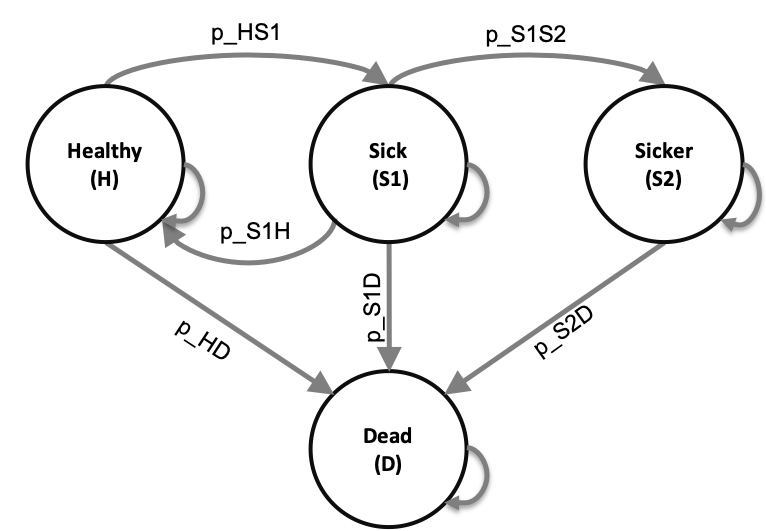
\includegraphics[width=10.64in]{figs/Sick-Sicker} 

}

\caption{State-transition diagram of the Sick-Sicker cohort state-transition model with the name of the health states and possible transitions with their corresponding transition probability names.}\label{fig:STD-Sick-Sicker}
\end{figure}

The model simulates the health care costs and quality-adjusted life-years (QALYs) of a cohort of 25-year-old individuals at risk of developing a hypothetical disease that has two stages: ``Sick'' and ``Sicker''.\textsuperscript{\protect\hyperlink{ref-Enns2015e}{11}} We simulate the cohort of individuals who all start in the ``Healthy'' state (denoted by ``H'') over their lifetime, which means that we will simulate the cohort for 75 cycles. The total number of cycles is denoted as \(n_T\) and defined in R as \texttt{n\_cycles}. In the accompanying tutorial, healthy individuals face a constant risk of death. To illustrate simulation time dependency, here we assume that healthy individuals face age-specific background mortality, and those who become ill over time transition to the ``Sick'' state (denoted by ``S1''). Once healthy individuals get sick, they incur a one-time utility decrement of 0.01 (\texttt{du\_HS1}, a disutility of transitioning from H to S1) and a transition cost of \$1,000 (\texttt{ic\_HS1}) that reflects the acute impacts of developing the illness. The S1 state is associated with higher mortality, higher health care costs, and lower quality of life than the H state. Once in the S1 state, individuals may recover (returning to the H state), die (move to the D state), or progress further to the ``Sicker'' state (denoted by ``S2''), with further increases in mortality risk and health care costs and reduced quality of life. We assume that it is not possible to distinguish between individuals in S1 and S2. In the state-residence time-dependent model, the risk of progressing from S1 to S2 is a function of the duration of time spent in S1. Individuals in S1 and S2 face an increased hazard of death, compared to healthy individuals, in the form of a hazard ratio (HR) of 3 and 10, respectively, relative to the background age-specific mortality hazard rate. Once simulated individuals die, they transition to the absorbing D state, where they remain, and incur a one-time cost of \$2,000 (\texttt{ic\_D}) that reflects the expected acute care preceding death. All transitions between non-death states are assumed to be conditional on surviving each cycle. We simulated the evolution of the cohort in one-year discrete-time cycles.

We use this cSTM to evaluate the cost-effectiveness of four strategies: Strategy A, strategy B, a combination of A and B (strategy AB), and the standard of care (strategy SoC). Strategy A involves administering treatment A to individuals in S1 and S2 but only increases the QoL of individuals in S1 from 0.75 (utility without treatment, \texttt{u\_S1}) to 0.95 (utility with treatment A, \texttt{u\_trtA}) and costs \$12,000 per year (\texttt{c\_trtA}).\textsuperscript{\protect\hyperlink{ref-Krijkamp2018}{12}} This strategy does not impact the QoL of individuals in S2, nor does it change the risk of becoming sick or progressing through the sick states. Strategy B uses treatment B to reduce only the rate of Sick individuals progressing to the S2 state with a hazard ratio (HR) of 0.6 (\texttt{hr\_S1S2\_trtB}) and costs \$13,000 per year (\texttt{c\_trtB}) and does not affect QoL. Strategy AB involves administering both treatments A and B. We discount both costs and QALYs at an annual rate of 3\%. Model parameters and the corresponding R variable names are presented in Table \ref{tab:param-table} and follow the notation described in the DARTH coding framework.\textsuperscript{\protect\hyperlink{ref-Alarid-Escudero2019e}{13}}

Note that for strategy A, the model has the same structure and identical transition probabilities to SoC. The only difference is the added cost of the treatment for S1 or S2, and QoL increases for S1. After comparing the four strategies in terms of expected QALYs and costs, we calculate the incremental cost per QALY gained between non-dominated strategies.

\begin{longtable}[]{@{}
  >{\raggedright\arraybackslash}p{(\columnwidth - 6\tabcolsep) * \real{0.45}}
  >{\centering\arraybackslash}p{(\columnwidth - 6\tabcolsep) * \real{0.16}}
  >{\centering\arraybackslash}p{(\columnwidth - 6\tabcolsep) * \real{0.19}}
  >{\centering\arraybackslash}p{(\columnwidth - 6\tabcolsep) * \real{0.20}}@{}}
\caption{\label{tab:param-table} Description of parameters, their R variable name, base-case values and distribution.}\tabularnewline
\toprule
\textbf{Parameter} & \textbf{R name} & \textbf{Base-case} & \textbf{Distribution} \\
\midrule
\endfirsthead
\toprule
\textbf{Parameter} & \textbf{R name} & \textbf{Base-case} & \textbf{Distribution} \\
\midrule
\endhead
Number of cycles (\(n_{T}\)) & \texttt{n\_cycles} & 75 years & constant \\
Names of health states & \texttt{v\_names\_states} & H, S1, S2, D & constant \\
Annual discount rate for costs & \texttt{d\_c} & 3\% & constant \\
Annual discount rate for QALYs & \texttt{d\_e} & 3\% & constant \\
Number of PSA samples (\(K\)) & \texttt{n\_sim} & 1,000 & constant \\
Annual transition probabilities conditional on surviving & & & \\
- Disease onset (H to S1) & \texttt{p\_HS1} & 0.15 & beta(30, 170) \\
- Recovery (S1 to H) & \texttt{p\_S1H} & 0.5 & beta(60, 60) \\
- Time-independent disease progression (S1 to S2) & \texttt{p\_S1S2} & 0.105 & beta(84, 716) \\
- Time-dependent disease progression (S1 to S2) & \texttt{v\_p\_S1S2\_tunnels} & & \\
~~~~Weibull parameters & & & \\
~~~~~~~~Scale (\(\lambda\)) & \texttt{p\_S1S2\_scale} & 0.08 & lognormal(log(0.08), 0.02) \\
~~~~~~~~Shape (\(\gamma\)) & \texttt{p\_S1S2\_shape} & 1.10 & lognormal(log(1.10), 0.05) \\
Annual mortality & & & \\
- Age-dependent background mortality rate (H to D) & \texttt{v\_r\_HDage} & age-specific & constant \\
- Hazard ratio of death in S1 vs H & \texttt{hr\_S1} & 3.0 & lognormal(log(3.0), 0.01) \\
- Hazard ratio of death in S2 vs H & \texttt{hr\_S2} & 10.0 & lognormal(log(10.0), 0.02) \\
Annual costs & & & \\
- Healthy individuals & \texttt{c\_H} & \$2,000 & gamma(100.0, 20.0) \\
- Sick individuals in S1 & \texttt{c\_S1} & \$4,000 & gamma(177.8, 22.5) \\
- Sick individuals in S2 & \texttt{c\_S2} & \$15,000 & gamma(225.0, 66.7) \\
- Dead individuals & \texttt{c\_D} & \$0 & - \\
- Cost of treatment A as an additional costs on individuals treated in S1 or S2 & \texttt{c\_trtA} & \$12,000 & gamma(576.0, 20.8) \\
- Cost of treatment B as an additional costs on individuals treated in S1 or S2 & \texttt{c\_trtB} & \$13,000 & gamma(676.0, 19.2) \\
Utility weights & & & \\
- Healthy individuals & \texttt{u\_H} & 1.00 & beta(200, 3) \\
- Sick individuals in S1 & \texttt{u\_S1} & 0.75 & beta(130, 45) \\
- Sick individuals in S2 & \texttt{u\_S2} & 0.50 & beta(230, 230) \\
- Dead individuals & \texttt{u\_D} & 0.00 & constant \\
Treatment A effectiveness & & & \\
- Utility for treated individuals in S1 & \texttt{u\_trtA} & 0.95 & beta(300, 15) \\
Treatment B effectiveness & & & \\
- Reduction in rate of disease progression (S1 to S2) as hazard ratio (HR) & \texttt{hr\_S1S2\_trtB} & log(0.6) & lognormal(log(0.6), 0.1) \\
Transition rewards & & & \\
- Utility decrement of healthy individuals & \texttt{du\_HS1} & 0.01 & beta(11,1088) \\
when transitioning to S1 & & & \\
- Cost of healthy individuals & \texttt{ic\_HS1} & \$1,000 & gamma(25, 40) \\
when transitioning to S1 & & & \\
- Cost of dying when transitioning to D & \texttt{ic\_D} & \$2,000 & gamma(100, 20) \\
\bottomrule
\end{longtable}

The R code below describes the initialization of the input parameters.

\begin{Shaded}
\begin{Highlighting}[]
\DocumentationTok{\#\# General setup}
\NormalTok{cycle\_length }\OtherTok{\textless{}{-}} \DecValTok{1} \CommentTok{\# cycle length equal one year}
\NormalTok{n\_age\_init }\OtherTok{\textless{}{-}} \DecValTok{25}  \CommentTok{\# age at baseline}
\NormalTok{n\_age\_max  }\OtherTok{\textless{}{-}} \DecValTok{100} \CommentTok{\# maximum age of follow up}
\NormalTok{n\_cycles }\OtherTok{\textless{}{-}}\NormalTok{ n\_age\_max }\SpecialCharTok{{-}}\NormalTok{ n\_age\_init }\CommentTok{\# number of cycles}
\CommentTok{\# The 4 health states of the model:}
\NormalTok{v\_names\_states }\OtherTok{\textless{}{-}} \FunctionTok{c}\NormalTok{(}\StringTok{"H"}\NormalTok{,  }\CommentTok{\# Healthy (H)}
                    \StringTok{"S1"}\NormalTok{, }\CommentTok{\# Sick (S1)}
                    \StringTok{"S2"}\NormalTok{, }\CommentTok{\# Sicker (S2)}
                    \StringTok{"D"}\NormalTok{)  }\CommentTok{\# Dead (D)}
\NormalTok{n\_states }\OtherTok{\textless{}{-}} \FunctionTok{length}\NormalTok{(v\_names\_states) }\CommentTok{\# number of health states }
\NormalTok{d\_e }\OtherTok{\textless{}{-}} \FloatTok{0.03} \CommentTok{\# discount rate for QALYs of 3\% per cycle }
\NormalTok{d\_c }\OtherTok{\textless{}{-}} \FloatTok{0.03} \CommentTok{\# discount rate for costs of 3\% per cycle }
\NormalTok{v\_names\_str }\OtherTok{\textless{}{-}} \FunctionTok{c}\NormalTok{(}\StringTok{"Standard of care"}\NormalTok{, }\CommentTok{\# store the strategy names}
                 \StringTok{"Strategy A"}\NormalTok{, }
                 \StringTok{"Strategy B"}\NormalTok{,}
                 \StringTok{"Strategy AB"}\NormalTok{) }

\DocumentationTok{\#\# Transition probabilities (per cycle), hazard ratios and odds ratio (OR)}
\NormalTok{p\_HS1   }\OtherTok{\textless{}{-}} \FloatTok{0.15}  \CommentTok{\# probability of becoming Sick when Healthy}
\NormalTok{p\_S1H   }\OtherTok{\textless{}{-}} \FloatTok{0.5}   \CommentTok{\# probability of becoming Healthy when Sick}
\NormalTok{p\_S1S2  }\OtherTok{\textless{}{-}} \FloatTok{0.105} \CommentTok{\# probability of becoming Sicker when Sick}
\NormalTok{hr\_S1   }\OtherTok{\textless{}{-}} \DecValTok{3}     \CommentTok{\# hazard ratio of death in Sick vs Healthy}
\NormalTok{hr\_S2   }\OtherTok{\textless{}{-}} \DecValTok{10}    \CommentTok{\# hazard ratio of death in Sicker vs Healthy }

\CommentTok{\# Effectiveness of treatment B}
\NormalTok{hr\_S1S2\_trtB }\OtherTok{\textless{}{-}} \FloatTok{0.6} \CommentTok{\# hazard ratio of becoming Sicker when Sick under treatment B}

\DocumentationTok{\#\# State rewards}
\DocumentationTok{\#\# Costs}
\NormalTok{c\_H    }\OtherTok{\textless{}{-}} \DecValTok{2000}  \CommentTok{\# cost of being Healthy for one cycle }
\NormalTok{c\_S1   }\OtherTok{\textless{}{-}} \DecValTok{4000}  \CommentTok{\# cost of being Sick for one cycle }
\NormalTok{c\_S2   }\OtherTok{\textless{}{-}} \DecValTok{15000} \CommentTok{\# cost of being Sicker for one cycle}
\NormalTok{c\_D    }\OtherTok{\textless{}{-}} \DecValTok{0}     \CommentTok{\# cost of being dead for one cycle}
\NormalTok{c\_trtA }\OtherTok{\textless{}{-}} \DecValTok{12000} \CommentTok{\# cost of receiving treatment A for one cycle}
\NormalTok{c\_trtB }\OtherTok{\textless{}{-}} \DecValTok{13000} \CommentTok{\# cost of receiving treatment B for one cycle }
\CommentTok{\# Utilities}
\NormalTok{u\_H    }\OtherTok{\textless{}{-}} \DecValTok{1}     \CommentTok{\# utility of being Healthy for one cycle }
\NormalTok{u\_S1   }\OtherTok{\textless{}{-}} \FloatTok{0.75}  \CommentTok{\# utility of being Sick for one cycle }
\NormalTok{u\_S2   }\OtherTok{\textless{}{-}} \FloatTok{0.5}   \CommentTok{\# utility of being Sicker for one cycle}
\NormalTok{u\_D    }\OtherTok{\textless{}{-}} \DecValTok{0}     \CommentTok{\# utility of being dead for one cycle}
\NormalTok{u\_trtA }\OtherTok{\textless{}{-}} \FloatTok{0.95}  \CommentTok{\# utility when receiving treatment A for one cycle}

\DocumentationTok{\#\# Transition rewards}
\NormalTok{du\_HS1 }\OtherTok{\textless{}{-}} \FloatTok{0.01}  \CommentTok{\# one{-}time utility decrement when transitioning from Healthy to Sick}
\NormalTok{ic\_HS1 }\OtherTok{\textless{}{-}} \DecValTok{1000}  \CommentTok{\# one{-}time cost when transitioning from Healthy to Sick}
\NormalTok{ic\_D   }\OtherTok{\textless{}{-}} \DecValTok{2000}  \CommentTok{\# one{-}time cost when dying}
\end{Highlighting}
\end{Shaded}

\hypertarget{simulation-time-dependency-1}{%
\subsection{Simulation-time dependency}\label{simulation-time-dependency-1}}

To illustrate the implementation of simulation-time dependency in the Sick-Sicker cSTM, we model all-cause mortality as a function of age. We obtain all-cause mortality from life tables in the form of age-specific mortality hazard rates, \(\mu(a)\), where \(a\) refers to age. For this example, we create a vector \texttt{v\_r\_mort\_by\_age} with age-specific background mortality hazard rates for 0 to 100 year-olds obtained from US life-tables.\textsuperscript{\protect\hyperlink{ref-Arias2017}{14}} To compute the transition probability from state H to state D, corresponding to cohort's age at each cycle, we transform the rate \(\mu(a)\) to a transition probability assuming a constant exponential hazard rate within each year of age
\[
  p_{[H,D,t]} = 1-\exp\left\{{-\mu(a_0 + t)}\right\},
\]
where \(a_0 =\) 25 is the starting age of the cohort. Instead of iterating through the mortality hazard rates, we obtain a vector of background mortality hazard rates for the ages of interest between 25 through 100 by subsetting \(\mu(a)\) (R variable name \texttt{v\_r\_mort\_by\_age}) for these ages. We transform the resulting R variable, \texttt{v\_r\_HDage}, to a probability.

\begin{Shaded}
\begin{Highlighting}[]
\CommentTok{\# Age{-}specific mortality rate in the Healthy state (background mortality)}
\NormalTok{v\_r\_HDage }\OtherTok{\textless{}{-}}\NormalTok{ v\_r\_mort\_by\_age[(n\_age\_init }\SpecialCharTok{+} \DecValTok{1}\NormalTok{) }\SpecialCharTok{+} \DecValTok{0}\SpecialCharTok{:}\NormalTok{(n\_cycles }\SpecialCharTok{{-}} \DecValTok{1}\NormalTok{)]}
\CommentTok{\# Transform to age{-}specific background mortality risk}
\NormalTok{v\_p\_HDage  }\OtherTok{\textless{}{-}} \DecValTok{1} \SpecialCharTok{{-}} \FunctionTok{exp}\NormalTok{(}\SpecialCharTok{{-}}\NormalTok{v\_r\_HDage) }
\end{Highlighting}
\end{Shaded}

Because mortality in S1 and S2 are relative to background mortality, adding age dependency to background mortality results in age-dependent mortality in S1 and S2 as well as in H. To generate the age-specific mortality in S1 and S2, we multiply the age-specific background mortality rate, \texttt{v\_r\_HDage}, by the constant hazard ratios \texttt{hr\_S1} and \texttt{hr\_S2}, respectively. We then convert the resulting age-specific mortality rates to probabilities.

\begin{Shaded}
\begin{Highlighting}[]
\DocumentationTok{\#\# Age{-}specific mortality rates in the Sick and Sicker states}
\NormalTok{v\_r\_S1Dage }\OtherTok{\textless{}{-}}\NormalTok{ v\_r\_HDage }\SpecialCharTok{*}\NormalTok{ hr\_S1 }\CommentTok{\# when Sick}
\NormalTok{v\_r\_S2Dage }\OtherTok{\textless{}{-}}\NormalTok{ v\_r\_HDage }\SpecialCharTok{*}\NormalTok{ hr\_S2 }\CommentTok{\# when Sicker}
\DocumentationTok{\#\# Age{-}specific probabilities of dying in the Sick and Sicker states}
\NormalTok{v\_p\_S1Dage }\OtherTok{\textless{}{-}} \DecValTok{1} \SpecialCharTok{{-}} \FunctionTok{exp}\NormalTok{(}\SpecialCharTok{{-}}\NormalTok{v\_r\_S1Dage) }\CommentTok{\# when Sick}
\NormalTok{v\_p\_S2Dage }\OtherTok{\textless{}{-}} \DecValTok{1} \SpecialCharTok{{-}} \FunctionTok{exp}\NormalTok{(}\SpecialCharTok{{-}}\NormalTok{v\_r\_S2Dage) }\CommentTok{\# when Sicker}
\end{Highlighting}
\end{Shaded}

To incorporate simulation-time dependency into the transition probability matrix, we expand the dimensions of the matrix and create a 3-dimensional transition probability array, \(\mathbf{P}\) and \texttt{a\_P} in R, of dimensions \(n_S \times n_S \times n_T\). The first two dimensions of this array correspond to transitions between states and the third dimension to time. The \(t\)-th element in the third dimension corresponds to the transition probability matrix at cycle \(t\). A visual representation of \texttt{a\_P} is shown in Figure \ref{fig:Array-Time-Dependent}.

\begin{figure}[H]

{\centering 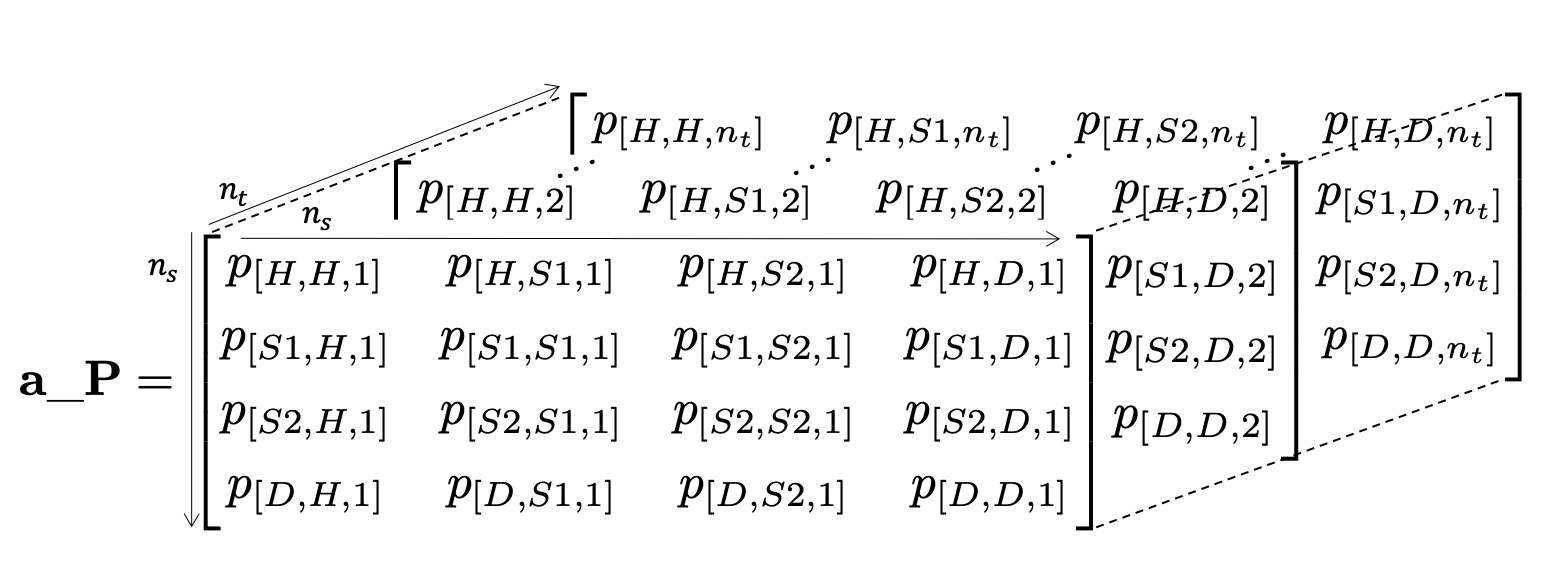
\includegraphics[width=1\linewidth]{figs/3D-state-transition-array-sick-sicker-without-tunnels} 

}

\caption{A 3-dimensional representation of the transition probability array of the Sick-Sicker model with simulation-time dependency.}\label{fig:Array-Time-Dependent}
\end{figure}

First, we initialize the transition probability array for SoC, \texttt{a\_P\_SoC}, with a default value of zero for all transition probabilities.

\begin{Shaded}
\begin{Highlighting}[]
\CommentTok{\# Initialize the transition probability array}
\NormalTok{a\_P\_SoC }\OtherTok{\textless{}{-}} \FunctionTok{array}\NormalTok{(}\DecValTok{0}\NormalTok{, }\AttributeTok{dim =} \FunctionTok{c}\NormalTok{(n\_states, n\_states, n\_cycles),}
              \AttributeTok{dimnames =} \FunctionTok{list}\NormalTok{(v\_names\_states, v\_names\_states, }\DecValTok{0}\SpecialCharTok{:}\NormalTok{(n\_cycles }\SpecialCharTok{{-}} \DecValTok{1}\NormalTok{)))}
\end{Highlighting}
\end{Shaded}

Filling \texttt{a\_P\_SoC} with the corresponding transition probabilities of the cohort under the SoC strategy is comparable with filling \texttt{m\_P} for a time-independent cSTM, accounting for the time dimension, which is represented by the third dimension of the array. However, this requires a slight modification of the code from the time-independent cSTM. The code below illustrates how to assign age-dependent transition probabilities in the third dimension of the array. For constant transitions over time, we only need to provide one value for the transition probability. R replicates the value of such transitions as many times as the number of cycles (\(n_T+1\) times in our example). We create the transition probability array for strategy A as a copy of SoC's because treatment A does not alter the cohort's transition probabilities.

\begin{Shaded}
\begin{Highlighting}[]
\DocumentationTok{\#\#\# Fill in array}
\DocumentationTok{\#\# From H}
\NormalTok{a\_P\_SoC[}\StringTok{"H"}\NormalTok{, }\StringTok{"H"}\NormalTok{, ]   }\OtherTok{\textless{}{-}}\NormalTok{ (}\DecValTok{1} \SpecialCharTok{{-}}\NormalTok{ v\_p\_HDage) }\SpecialCharTok{*}\NormalTok{ (}\DecValTok{1} \SpecialCharTok{{-}}\NormalTok{ p\_HS1)}
\NormalTok{a\_P\_SoC[}\StringTok{"H"}\NormalTok{, }\StringTok{"S1"}\NormalTok{, ]  }\OtherTok{\textless{}{-}}\NormalTok{ (}\DecValTok{1} \SpecialCharTok{{-}}\NormalTok{ v\_p\_HDage) }\SpecialCharTok{*}\NormalTok{ p\_HS1}
\NormalTok{a\_P\_SoC[}\StringTok{"H"}\NormalTok{, }\StringTok{"D"}\NormalTok{, ]   }\OtherTok{\textless{}{-}}\NormalTok{ v\_p\_HDage}
\DocumentationTok{\#\# From S1}
\NormalTok{a\_P\_SoC[}\StringTok{"S1"}\NormalTok{, }\StringTok{"H"}\NormalTok{, ]  }\OtherTok{\textless{}{-}}\NormalTok{ (}\DecValTok{1} \SpecialCharTok{{-}}\NormalTok{ v\_p\_S1Dage) }\SpecialCharTok{*}\NormalTok{ p\_S1H}
\NormalTok{a\_P\_SoC[}\StringTok{"S1"}\NormalTok{, }\StringTok{"S1"}\NormalTok{, ] }\OtherTok{\textless{}{-}}\NormalTok{ (}\DecValTok{1} \SpecialCharTok{{-}}\NormalTok{ v\_p\_S1Dage) }\SpecialCharTok{*}\NormalTok{ (}\DecValTok{1} \SpecialCharTok{{-}}\NormalTok{ (p\_S1H }\SpecialCharTok{+}\NormalTok{ p\_S1S2))}
\NormalTok{a\_P\_SoC[}\StringTok{"S1"}\NormalTok{, }\StringTok{"S2"}\NormalTok{, ] }\OtherTok{\textless{}{-}}\NormalTok{ (}\DecValTok{1} \SpecialCharTok{{-}}\NormalTok{ v\_p\_S1Dage) }\SpecialCharTok{*}\NormalTok{ p\_S1S2}
\NormalTok{a\_P\_SoC[}\StringTok{"S1"}\NormalTok{, }\StringTok{"D"}\NormalTok{, ]  }\OtherTok{\textless{}{-}}\NormalTok{ v\_p\_S1Dage}
\DocumentationTok{\#\# From S2}
\NormalTok{a\_P\_SoC[}\StringTok{"S2"}\NormalTok{, }\StringTok{"S2"}\NormalTok{, ] }\OtherTok{\textless{}{-}} \DecValTok{1} \SpecialCharTok{{-}}\NormalTok{ v\_p\_S2Dage}
\NormalTok{a\_P\_SoC[}\StringTok{"S2"}\NormalTok{, }\StringTok{"D"}\NormalTok{, ]  }\OtherTok{\textless{}{-}}\NormalTok{ v\_p\_S2Dage}
\DocumentationTok{\#\# From D}
\NormalTok{a\_P\_SoC[}\StringTok{"D"}\NormalTok{, }\StringTok{"D"}\NormalTok{, ]   }\OtherTok{\textless{}{-}} \DecValTok{1}

\DocumentationTok{\#\# Initialize transition probability matrix for strategy A as a copy of SoC\textquotesingle{}s}
\NormalTok{a\_P\_strA }\OtherTok{\textless{}{-}}\NormalTok{ a\_P\_SoC}
\end{Highlighting}
\end{Shaded}

As mentioned above, each slice along the third dimension of \texttt{a\_P\_SoC} corresponds to a transition probability matrix. For example, the transition matrix for 25-year-olds in the Sick-Sicker model under the SoC strategy can be retrieved using:

\begin{Shaded}
\begin{Highlighting}[]
\NormalTok{a\_P\_SoC[, , }\DecValTok{1}\NormalTok{]}
\end{Highlighting}
\end{Shaded}

\begin{verbatim}
##            H        S1        S2           D
## H  0.8491385 0.1498480 0.0000000 0.001013486
## S1 0.4984813 0.3938002 0.1046811 0.003037378
## S2 0.0000000 0.0000000 0.9899112 0.010088764
## D  0.0000000 0.0000000 0.0000000 1.000000000
\end{verbatim}

Similar to the time-independent cSTM, treatment A does not change the transition probabilities. For treatment B, we first initialize the three-dimensional array of transition probabilities, \texttt{a\_P\_strB} as a copy of \texttt{a\_P\_SoC} and update only the probability of remaining in S1 and the transition probability from S1 to S2 (i.e., \texttt{p\_S1S2} is replaced with \texttt{p\_S1S2\_trtB}).

\begin{Shaded}
\begin{Highlighting}[]
\DocumentationTok{\#\# Initialize transition probability array for strategy B}
\NormalTok{a\_P\_strB }\OtherTok{\textless{}{-}}\NormalTok{ a\_P\_SoC}
\DocumentationTok{\#\# Update only transition probabilities from S1 involving p\_S1S2}
\NormalTok{a\_P\_strB[}\StringTok{"S1"}\NormalTok{, }\StringTok{"S1"}\NormalTok{, ] }\OtherTok{\textless{}{-}}\NormalTok{ (}\DecValTok{1} \SpecialCharTok{{-}}\NormalTok{ v\_p\_S1Dage) }\SpecialCharTok{*}\NormalTok{ (}\DecValTok{1} \SpecialCharTok{{-}}\NormalTok{ (p\_S1H }\SpecialCharTok{+}\NormalTok{ p\_S1S2\_trtB))}
\NormalTok{a\_P\_strB[}\StringTok{"S1"}\NormalTok{, }\StringTok{"S2"}\NormalTok{, ] }\OtherTok{\textless{}{-}}\NormalTok{ (}\DecValTok{1} \SpecialCharTok{{-}}\NormalTok{ v\_p\_S1Dage) }\SpecialCharTok{*}\NormalTok{ p\_S1S2\_trtB}

\DocumentationTok{\#\# Initialize transition probability matrix for strategy AB as a copy of B\textquotesingle{}s}
\NormalTok{a\_P\_strAB }\OtherTok{\textless{}{-}}\NormalTok{ a\_P\_strB}
\end{Highlighting}
\end{Shaded}

Once we create the transition probability arrays, we check they are valid (i.e., ensuring transition probabilities are between 0 and 1, and transition probabilities from each state sum to 1) using the functions \texttt{check\_sum\_of\_transition\_array} and \texttt{check\_transition\_probability}, provided in the \texttt{darthtools} package (\url{https://github.com/DARTH-git/darthtools}).

\begin{Shaded}
\begin{Highlighting}[]
\DocumentationTok{\#\#\# Check if transition probability matrices are valid}
\DocumentationTok{\#\# Check that transition probabilities are [0, 1]}
\FunctionTok{check\_transition\_probability}\NormalTok{(a\_P\_SoC)}
\FunctionTok{check\_transition\_probability}\NormalTok{(a\_P\_strA)}
\FunctionTok{check\_transition\_probability}\NormalTok{(a\_P\_strB)}
\FunctionTok{check\_transition\_probability}\NormalTok{(a\_P\_strAB)}
\DocumentationTok{\#\# Check that all rows sum to 1}
\FunctionTok{check\_sum\_of\_transition\_array}\NormalTok{(a\_P\_SoC, }\AttributeTok{n\_states =}\NormalTok{ n\_states, }\AttributeTok{n\_cycles =}\NormalTok{ n\_cycles)}
\FunctionTok{check\_sum\_of\_transition\_array}\NormalTok{(a\_P\_strA, }\AttributeTok{n\_states =}\NormalTok{ n\_states, }\AttributeTok{n\_cycles =}\NormalTok{ n\_cycles)}
\FunctionTok{check\_sum\_of\_transition\_array}\NormalTok{(a\_P\_strB, }\AttributeTok{n\_states =}\NormalTok{ n\_states, }\AttributeTok{n\_cycles =}\NormalTok{ n\_cycles)}
\FunctionTok{check\_sum\_of\_transition\_array}\NormalTok{(a\_P\_strAB, }\AttributeTok{n\_states =}\NormalTok{ n\_states, }\AttributeTok{n\_cycles =}\NormalTok{ n\_cycles)}
\end{Highlighting}
\end{Shaded}

In the Sick-Sicker model, the entire cohort starts in the Healthy state. Therefore, we create the \(1 \times n_S\) initial state vector \texttt{v\_s\_init} with all of the cohort assigned to the H state:

\begin{Shaded}
\begin{Highlighting}[]
\NormalTok{v\_s\_init }\OtherTok{\textless{}{-}} \FunctionTok{c}\NormalTok{(}\AttributeTok{H =} \DecValTok{1}\NormalTok{, }\AttributeTok{S1 =} \DecValTok{0}\NormalTok{, }\AttributeTok{S2 =} \DecValTok{0}\NormalTok{, }\AttributeTok{D =} \DecValTok{0}\NormalTok{) }\CommentTok{\# initial state vector}
\NormalTok{v\_s\_init}
\CommentTok{\#  H S1 S2  D }
\CommentTok{\#  1  0  0  0}
\end{Highlighting}
\end{Shaded}

We use the variable \texttt{v\_s\_init} to initialize \(M\) represented by \texttt{m\_M} for the cohort under SoC strategy. We also create a trace for each of the other treatment-based strategies. Note that the initial state vector, \texttt{v\_s\_init}, can be modified to account for the distribution of the cohort across the states at the start of the simulation and might vary by strategy. To simulate the cohort over the \(n_T\) cycles for the simulation-time-dependent cSTM, we initialize four cohort trace matrices.

\begin{Shaded}
\begin{Highlighting}[]
\DocumentationTok{\#\# Initialize cohort trace for age{-}dependent cSTM under SoC}
\NormalTok{m\_M\_SoC }\OtherTok{\textless{}{-}} \FunctionTok{matrix}\NormalTok{(}\ConstantTok{NA}\NormalTok{, }
                 \AttributeTok{nrow =}\NormalTok{ (n\_cycles }\SpecialCharTok{+} \DecValTok{1}\NormalTok{), }\AttributeTok{ncol =}\NormalTok{ n\_states, }
                 \AttributeTok{dimnames =} \FunctionTok{list}\NormalTok{(}\DecValTok{0}\SpecialCharTok{:}\NormalTok{n\_cycles, v\_names\_states))}
\CommentTok{\# Store the initial state vector in the first row of the cohort trace}
\NormalTok{m\_M\_SoC[}\DecValTok{1}\NormalTok{, ] }\OtherTok{\textless{}{-}}\NormalTok{ v\_s\_init}
\DocumentationTok{\#\# Initialize cohort trace for strategies A, B, and AB}
\CommentTok{\# Structure and initial states are the same as for SoC}
\NormalTok{m\_M\_strA  }\OtherTok{\textless{}{-}}\NormalTok{ m\_M\_SoC }\CommentTok{\# Strategy A}
\NormalTok{m\_M\_strB  }\OtherTok{\textless{}{-}}\NormalTok{ m\_M\_SoC }\CommentTok{\# Strategy B}
\NormalTok{m\_M\_strAB }\OtherTok{\textless{}{-}}\NormalTok{ m\_M\_SoC }\CommentTok{\# Strategy AB}
\end{Highlighting}
\end{Shaded}

We then use the matrix product to get the state vector at cycle \(t\). This equation is similar to the one described for the time-independent model. The only modification required is to index the transition probability arrays by \(t\) to obtain each strategy's cycle-specific transition probability matrices.

\begin{Shaded}
\begin{Highlighting}[]
\CommentTok{\# Iterative solution of age{-}dependent cSTM}
\ControlFlowTok{for}\NormalTok{(t }\ControlFlowTok{in} \DecValTok{1}\SpecialCharTok{:}\NormalTok{n\_cycles)\{}
  \CommentTok{\# For SoC}
\NormalTok{  m\_M\_SoC[t }\SpecialCharTok{+} \DecValTok{1}\NormalTok{, ] }\OtherTok{\textless{}{-}}\NormalTok{ m\_M\_SoC[t, ] }\SpecialCharTok{\%*\%}\NormalTok{ a\_P\_SoC[, , t]}
  \CommentTok{\# For strategy A}
\NormalTok{  m\_M\_strA[t }\SpecialCharTok{+} \DecValTok{1}\NormalTok{, ] }\OtherTok{\textless{}{-}}\NormalTok{ m\_M\_strA[t, ] }\SpecialCharTok{\%*\%}\NormalTok{ a\_P\_strA[, , t]}
  \CommentTok{\# For strategy B}
\NormalTok{  m\_M\_strB[t }\SpecialCharTok{+} \DecValTok{1}\NormalTok{, ] }\OtherTok{\textless{}{-}}\NormalTok{ m\_M\_strB[t, ] }\SpecialCharTok{\%*\%}\NormalTok{ a\_P\_strB[, , t]}
  \CommentTok{\# For strategy AB}
\NormalTok{  m\_M\_strAB[t }\SpecialCharTok{+} \DecValTok{1}\NormalTok{, ] }\OtherTok{\textless{}{-}}\NormalTok{ m\_M\_strAB[t, ] }\SpecialCharTok{\%*\%}\NormalTok{ a\_P\_strAB[, , t]}
\NormalTok{\}}
\end{Highlighting}
\end{Shaded}

A graphical representation of the cohort trace for all cycles of the age-dependent cSTM under SoC is shown in Figure \ref{fig:Sick-Sicker-Trace-AgeDep}.

\begin{figure}[H]

{\centering 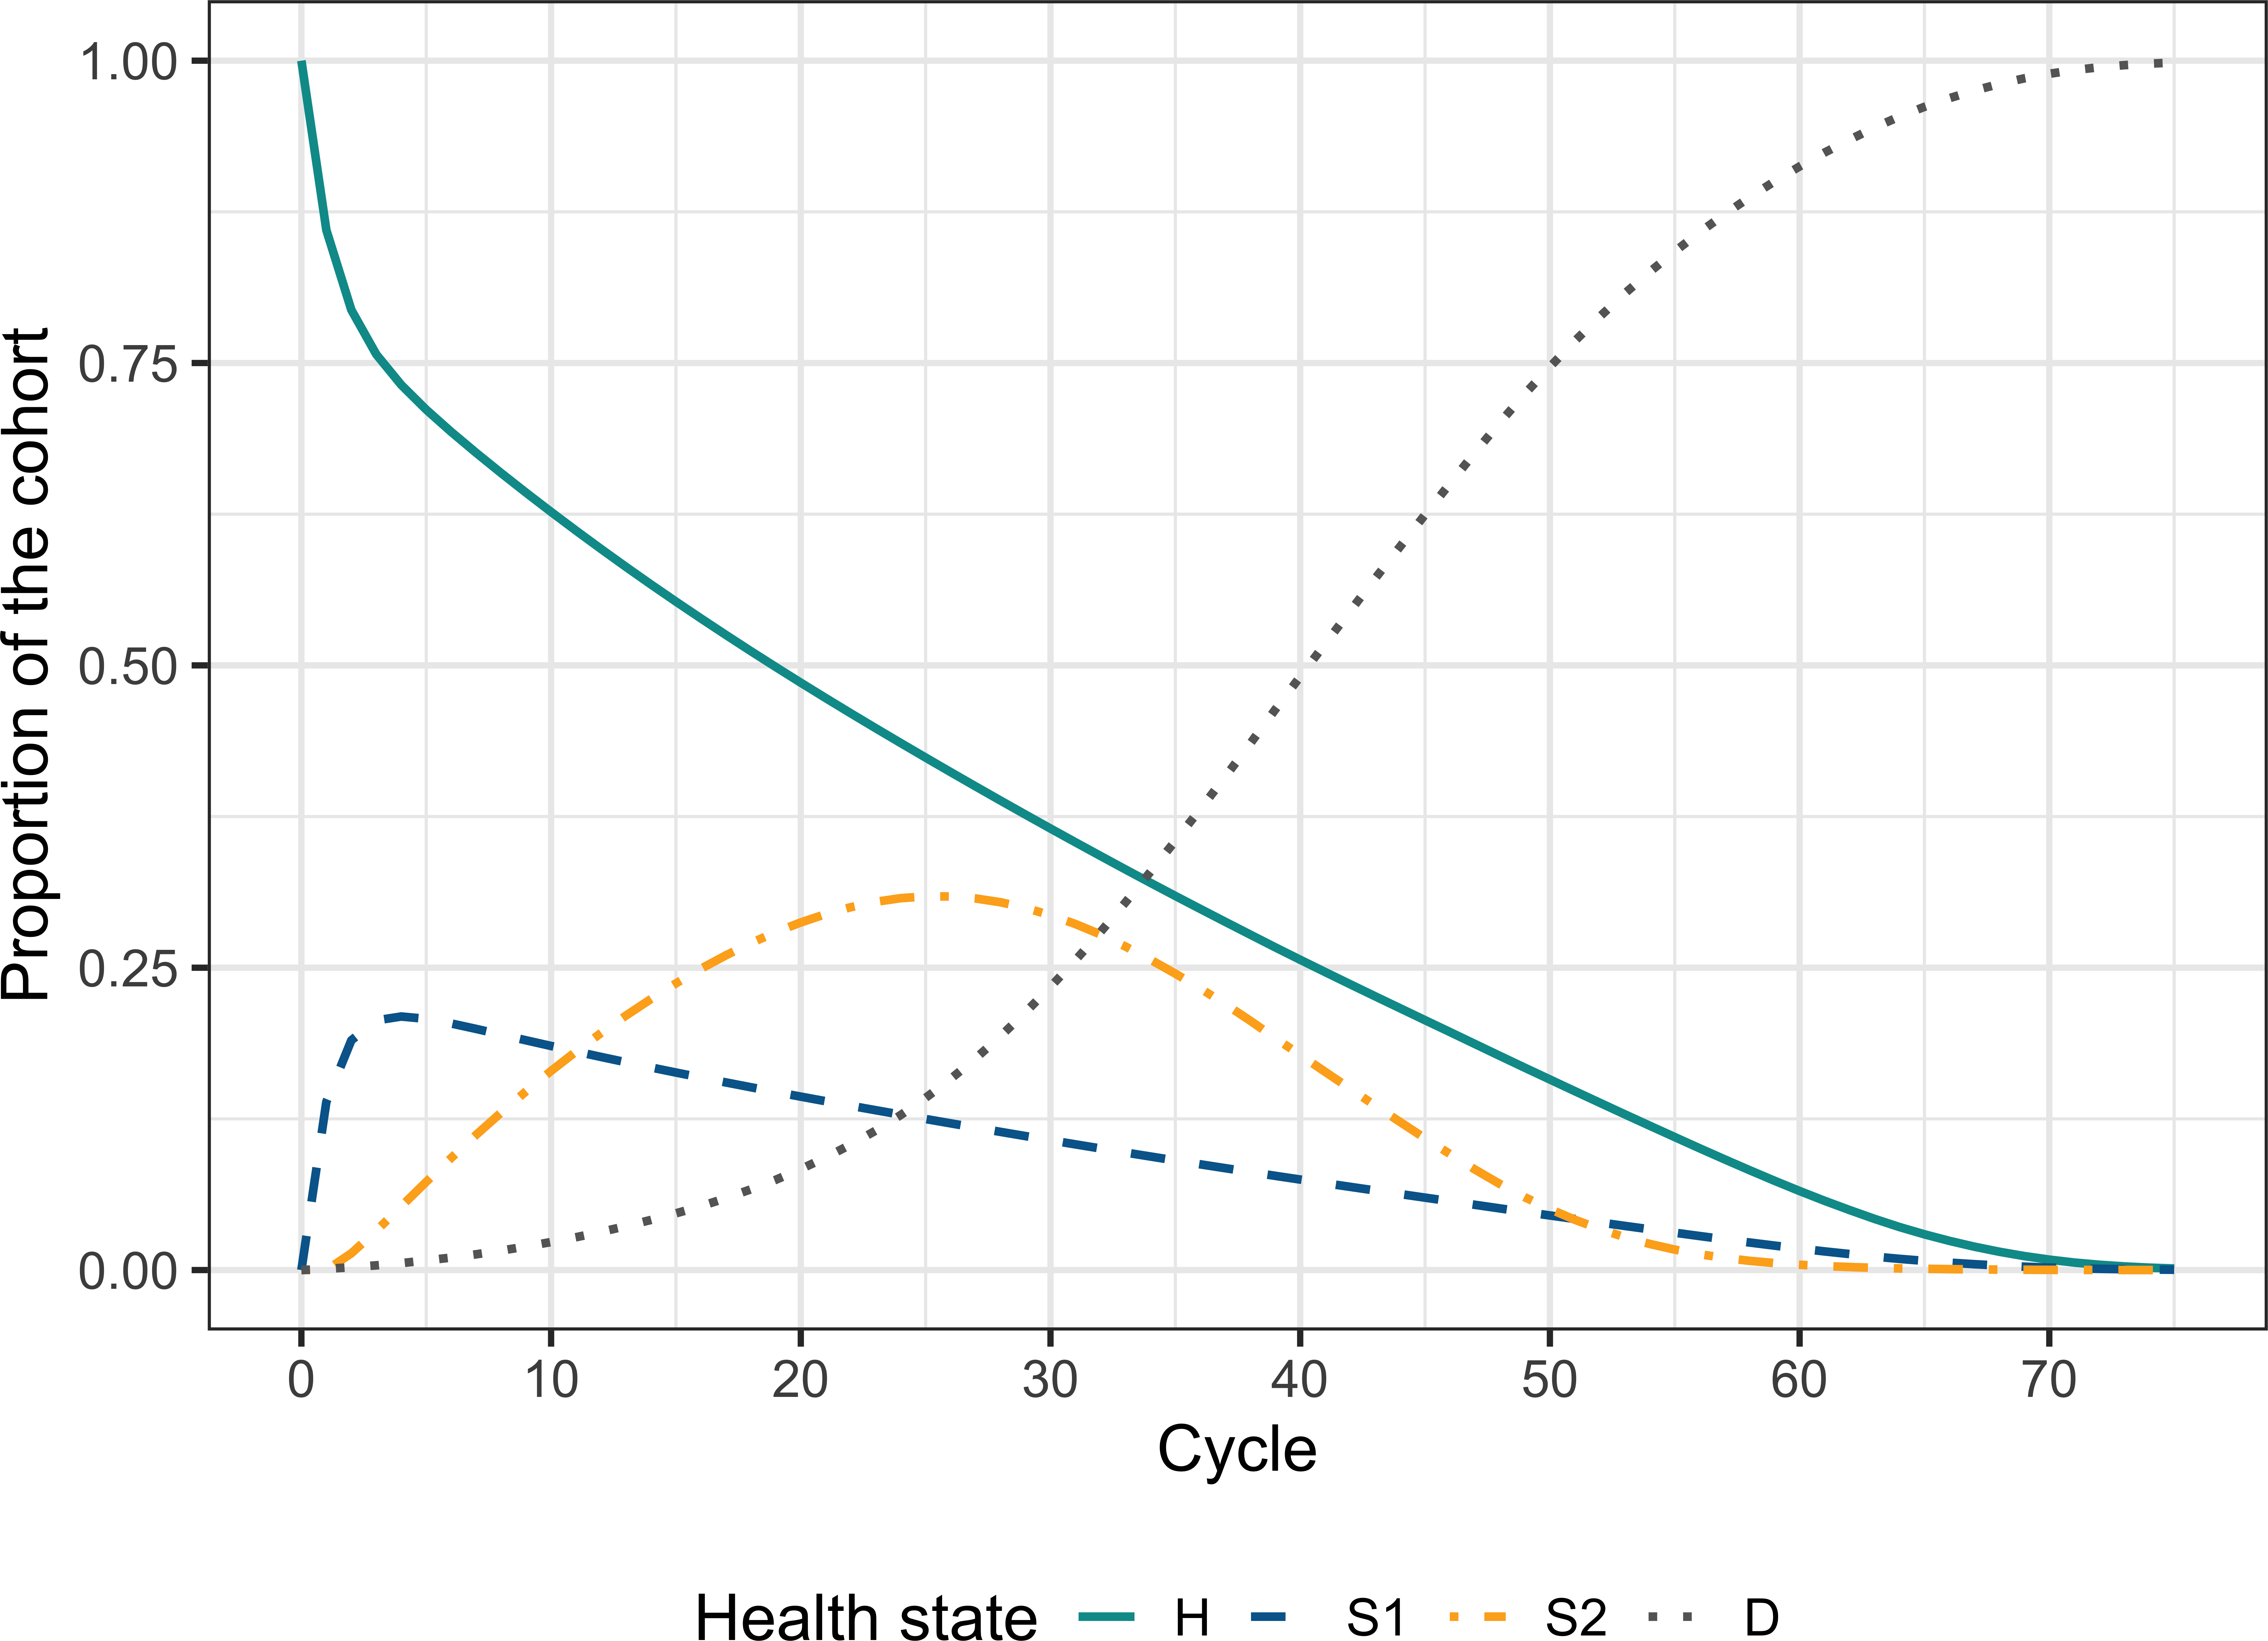
\includegraphics{figs/Sick-Sicker-Trace-AgeDep-1} 

}

\caption{Cohort trace of the age-dependent cSTM under strategies SoC and A.}\label{fig:Sick-Sicker-Trace-AgeDep}
\end{figure}

\hypertarget{time-dependency-on-state-residence-1}{%
\subsection{Time dependency on state residence}\label{time-dependency-on-state-residence-1}}

To add a state-residence dependency to the simulation-time-dependent Sick-Sicker model defined above, we assume the risk of progression from S1 to S2 increases as a function of the time \(\tau = 1, \ldots, n_{\text{tunnels}}\) the cohort remains in the S1 state. This increase follows a Weibull hazard function, \(h(\tau)\), defined as
\[
  h(\tau) = \gamma \lambda (\lambda \tau)^{\gamma-1},
\]
with a corresponding cumulative hazard, \(H(\tau)\),
\[
H(\tau) = (\lambda \tau)^{\gamma},
\]
where \(\lambda\) and \(\gamma\) are the scale and shape parameters of the Weibull function, respectively.

To derive a transition probability from S1 to S2 as a function as a function of the time the cohort spends in S1, \(p_{\left[S1_{\tau},S2, \tau\right]}\), from \(H(\tau)\), we use the following equation\textsuperscript{\protect\hyperlink{ref-Diaby2014}{15}}
\begin{equation}
p_{\left[S1_{\tau},S2, \tau\right]} = 1-\exp{(H(\tau-1) - H(\tau))}.
\label{eq:tp-from-H}
\end{equation}

Substituting the Weibull cumulative hazard in Equation \eqref{eq:tp-from-H}, the transition probability is \(p_{\left[S1_{\tau},S2, \tau\right]}\), is
\begin{equation}
p_{\left[S1_{\tau},S2, \tau\right]} = 1-\exp{((\lambda (\tau-1))^{\gamma} -  (\lambda \tau)^{\gamma})}.
\label{eq:tp-from-H-weibull}
\end{equation}

We assume that state-residence dependency affects the cohort in the S1 state throughout the whole simulation (i.e., \(n_{\text{tunnels}}=n_T\)) and create a new variable called \texttt{n\_tunnel\_size} with the length of the tunnel equal to \texttt{n\_cycles}. Thus, there will be 75 S1 tunnel states plus 3 more states (H, S2, D) resulting in a total of \(n_{S_{\text{tunnels}}}\) = 78.

Figure \ref{fig:STD-Sick-Sicker-tunnels} shows the Sick-Sicker model's state-transition diagram with state-residence dependency with \(n_{\text{tunnels}}\) tunnel states for S1.

\begin{figure}[H]

{\centering 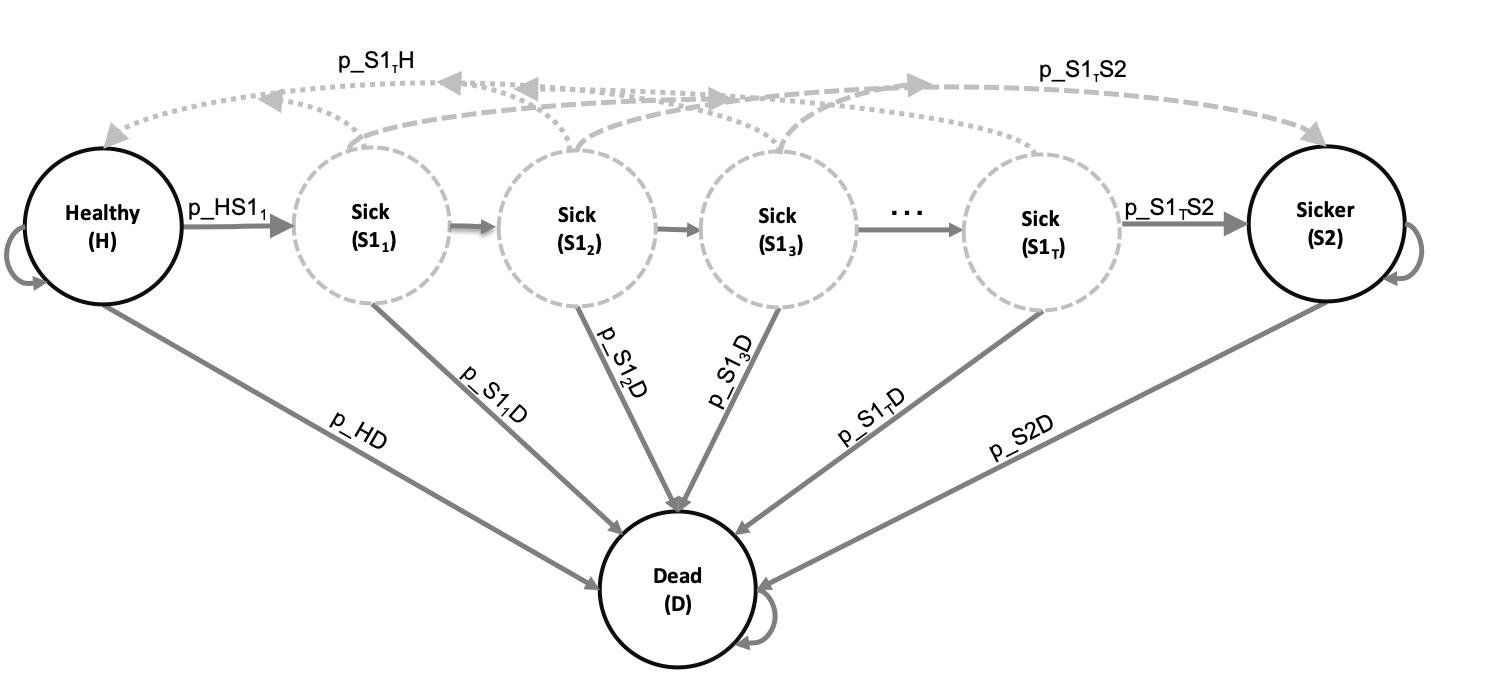
\includegraphics[width=1\linewidth]{figs/Sick-Sicker-with-tunnels} 

}

\caption{State-transition diagram of the Sick-Sicker model with tunnel states expanding the Sick state ($S1_1, S1_2,...,S1_{n_{ ext{tunnels}}}$).}\label{fig:STD-Sick-Sicker-tunnels}
\end{figure}

To implement state-residence dependency in the Sick-Sicker, we create the vector variables \texttt{v\_Sick\_tunnel} and \texttt{v\_names\_states\_tunnels} with the names of the Sick tunnel states' and all the states of the cSTM, including tunnels, respectively, and use the parameters listed in Table \ref{tab:Timedep-cSTM-components-table}.

\begin{Shaded}
\begin{Highlighting}[]
\DocumentationTok{\#\# Number of tunnels}
\NormalTok{n\_tunnel\_size }\OtherTok{\textless{}{-}}\NormalTok{ n\_cycles }
\DocumentationTok{\#\# Vector with cycles for tunnels}
\NormalTok{v\_cycles\_tunnel }\OtherTok{\textless{}{-}} \DecValTok{1}\SpecialCharTok{:}\NormalTok{n\_tunnel\_size}
\DocumentationTok{\#\# Vector with names for tunnel states of Sick state}
\NormalTok{v\_Sick\_tunnel }\OtherTok{\textless{}{-}} \FunctionTok{paste}\NormalTok{(}\StringTok{"S1\_"}\NormalTok{, }\FunctionTok{seq}\NormalTok{(}\DecValTok{1}\NormalTok{, n\_tunnel\_size), }\StringTok{"Yr"}\NormalTok{, }\AttributeTok{sep =} \StringTok{""}\NormalTok{)}
\DocumentationTok{\#\# Create variables for model with tunnels}
\NormalTok{v\_names\_states\_tunnels }\OtherTok{\textless{}{-}} \FunctionTok{c}\NormalTok{(}\StringTok{"H"}\NormalTok{, v\_Sick\_tunnel, }\StringTok{"S2"}\NormalTok{, }\StringTok{"D"}\NormalTok{) }\CommentTok{\# state names}
\NormalTok{n\_states\_tunnels }\OtherTok{\textless{}{-}} \FunctionTok{length}\NormalTok{(v\_names\_states\_tunnels)         }\CommentTok{\# number of states}
\DocumentationTok{\#\# Initialize first cycle of Markov trace accounting for the tunnels}
\NormalTok{v\_s\_init\_tunnels }\OtherTok{\textless{}{-}} \FunctionTok{c}\NormalTok{(}\DecValTok{1}\NormalTok{, }\FunctionTok{rep}\NormalTok{(}\DecValTok{0}\NormalTok{, n\_tunnel\_size), }\DecValTok{0}\NormalTok{, }\DecValTok{0}\NormalTok{) }
\end{Highlighting}
\end{Shaded}

Then, the transition probability dependent on state residence from Sick to Sicker, \texttt{v\_p\_S1S2\_tunnels}, based on a Weibull function in Equation \eqref{eq:tp-from-H-weibull} is:

\begin{Shaded}
\begin{Highlighting}[]
\CommentTok{\# Weibull parameters}
\NormalTok{p\_S1S2\_scale }\OtherTok{\textless{}{-}} \FloatTok{0.08} \CommentTok{\# scale}
\NormalTok{p\_S1S2\_shape }\OtherTok{\textless{}{-}} \FloatTok{1.1}  \CommentTok{\# shape}
\CommentTok{\# Weibull function}
\NormalTok{v\_p\_S1S2\_tunnels }\OtherTok{\textless{}{-}} \DecValTok{1}\SpecialCharTok{{-}}\FunctionTok{exp}\NormalTok{(((v\_cycles\_tunnel}\DecValTok{{-}1}\NormalTok{)}\SpecialCharTok{*}\NormalTok{p\_S1S2\_scale)}\SpecialCharTok{\^{}}\NormalTok{p\_S1S2\_shape }\SpecialCharTok{{-}} 
\NormalTok{                            (v\_cycles\_tunnel}\SpecialCharTok{*}\NormalTok{p\_S1S2\_scale)}\SpecialCharTok{\^{}}\NormalTok{p\_S1S2\_shape)}
\end{Highlighting}
\end{Shaded}

To adapt the 3-dimensional transition probability array to incorporate both age and state-residence dependence in the Sick-Sicker model under SoC, we first create an expanded 3-dimensional array accounting for tunnels, \texttt{a\_P\_tunnels\_SoC}. The dimensions of this array are \(n_{S_{\text{tunnels}}} \times n_{S_{\text{tunnels}}} \times n_T\). A visual representation of \texttt{a\_P\_tunnels\_SoC} of the Sick-Sicker model with tunnel states expanding the Sick state is shown in Figure \ref{fig:Array-Time-Dependent-Tunnels}.

\begin{Shaded}
\begin{Highlighting}[]
\CommentTok{\# Initialize array}
\NormalTok{a\_P\_tunnels\_SoC }\OtherTok{\textless{}{-}} \FunctionTok{array}\NormalTok{(}\DecValTok{0}\NormalTok{, }\AttributeTok{dim =} \FunctionTok{c}\NormalTok{(n\_states\_tunnels, n\_states\_tunnels, n\_cycles),}
                         \AttributeTok{dimnames =} \FunctionTok{list}\NormalTok{(v\_names\_states\_tunnels, }
\NormalTok{                                         v\_names\_states\_tunnels, }
                                         \DecValTok{0}\SpecialCharTok{:}\NormalTok{(n\_cycles }\SpecialCharTok{{-}} \DecValTok{1}\NormalTok{)))}
\end{Highlighting}
\end{Shaded}

\begin{figure}[H]

{\centering 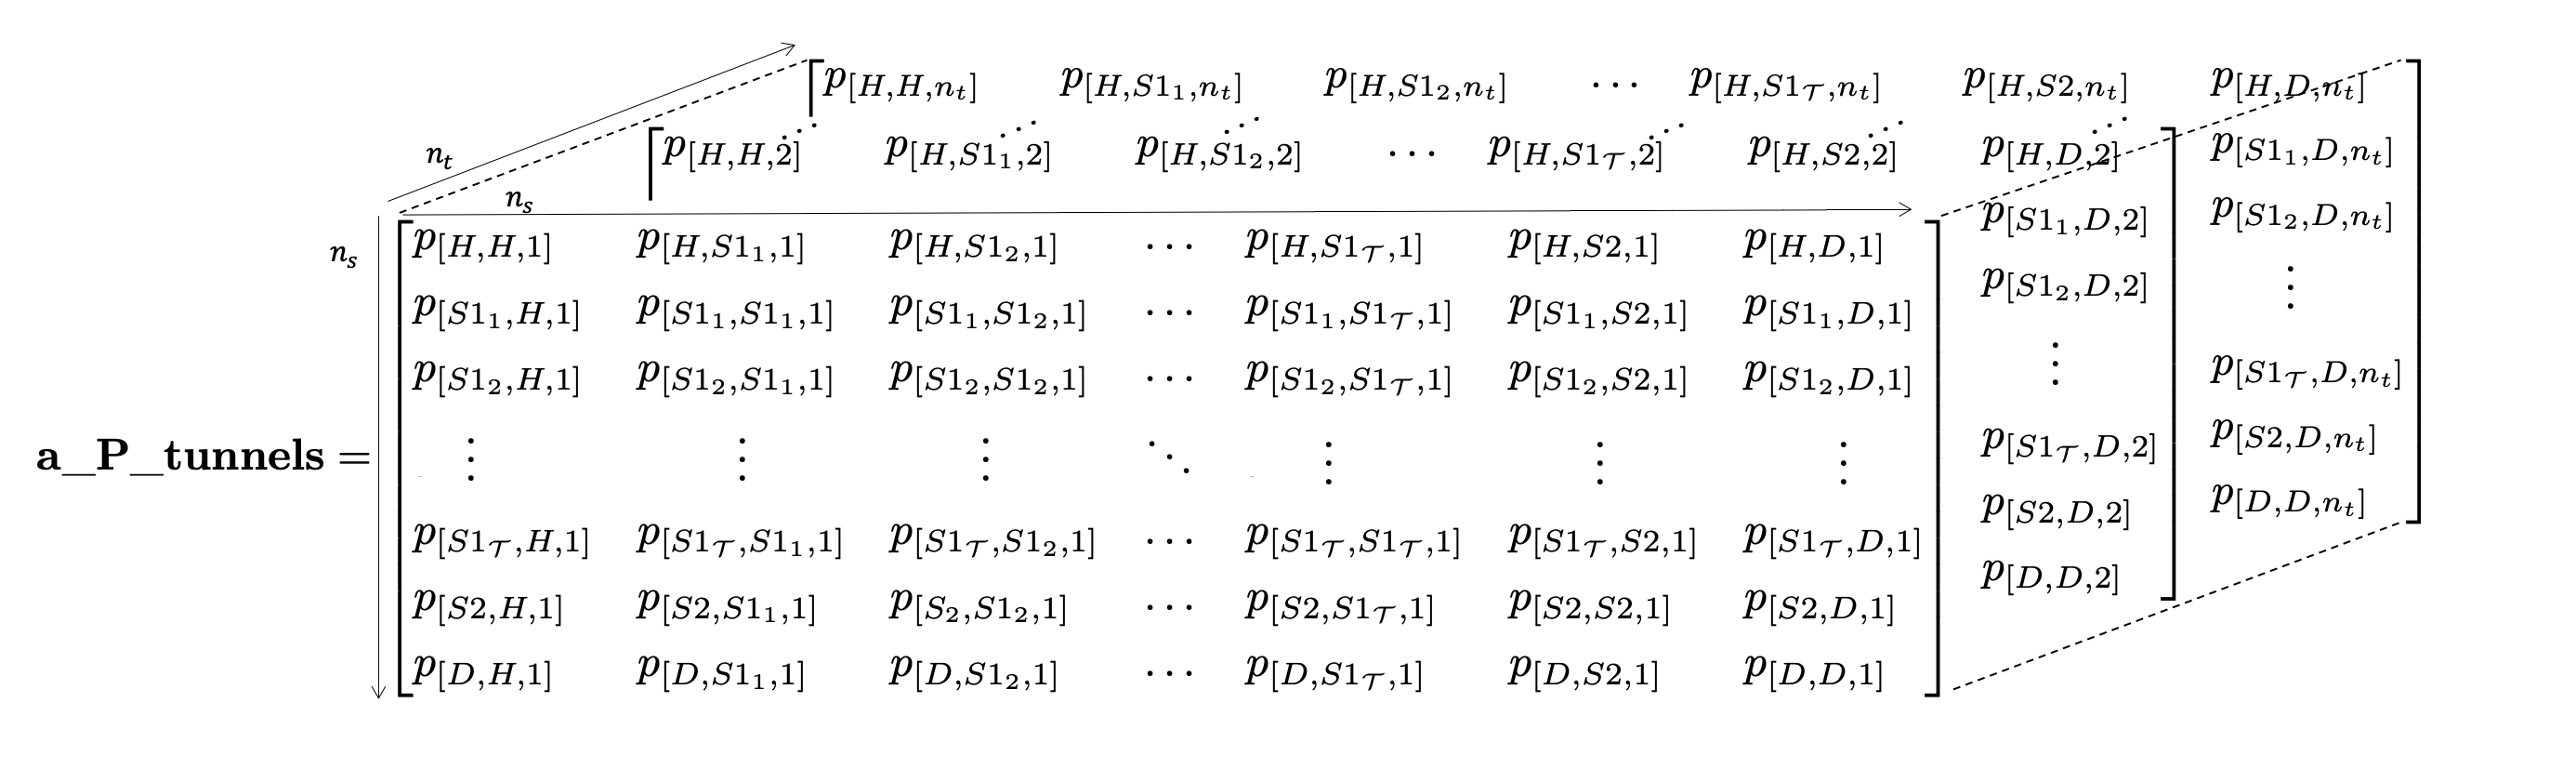
\includegraphics[width=1\linewidth]{figs/3D-state-transition-array-sick-sicker-tunnels} 

}

\caption{The 3-dimensional transition probability array of the Sick-Sicker model expanded to account for age-dependence and S1 state-residence using tunnel states.}\label{fig:Array-Time-Dependent-Tunnels}
\end{figure}

Filling \texttt{a\_P\_tunnels\_SoC} with the corresponding transition probabilities is similar to how it's done with \texttt{a\_P\_SoC} above, with the difference being that we now fill the transition probabilities from all the tunnel states by iterating through all the tunnel states and assigning the corresponding disease progression transition probabilities.

\begin{Shaded}
\begin{Highlighting}[]
\DocumentationTok{\#\#\# Fill in array}
\DocumentationTok{\#\# From H}
\NormalTok{a\_P\_tunnels\_SoC[}\StringTok{"H"}\NormalTok{, }\StringTok{"H"}\NormalTok{, ]              }\OtherTok{\textless{}{-}}\NormalTok{ (}\DecValTok{1} \SpecialCharTok{{-}}\NormalTok{ v\_p\_HDage) }\SpecialCharTok{*}\NormalTok{ (}\DecValTok{1} \SpecialCharTok{{-}}\NormalTok{ p\_HS1)}
\NormalTok{a\_P\_tunnels\_SoC[}\StringTok{"H"}\NormalTok{, v\_Sick\_tunnel[}\DecValTok{1}\NormalTok{], ] }\OtherTok{\textless{}{-}}\NormalTok{ (}\DecValTok{1} \SpecialCharTok{{-}}\NormalTok{ v\_p\_HDage) }\SpecialCharTok{*}\NormalTok{ p\_HS1}
\NormalTok{a\_P\_tunnels\_SoC[}\StringTok{"H"}\NormalTok{, }\StringTok{"D"}\NormalTok{, ]              }\OtherTok{\textless{}{-}}\NormalTok{ v\_p\_HDage}
\DocumentationTok{\#\# From S1}
\ControlFlowTok{for}\NormalTok{(i }\ControlFlowTok{in} \DecValTok{1}\SpecialCharTok{:}\NormalTok{(n\_tunnel\_size }\SpecialCharTok{{-}} \DecValTok{1}\NormalTok{))\{}
\NormalTok{  a\_P\_tunnels\_SoC[v\_Sick\_tunnel[i], }\StringTok{"H"}\NormalTok{, ]  }\OtherTok{\textless{}{-}}\NormalTok{ (}\DecValTok{1} \SpecialCharTok{{-}}\NormalTok{ v\_p\_S1Dage) }\SpecialCharTok{*}\NormalTok{ p\_S1H}
\NormalTok{  a\_P\_tunnels\_SoC[v\_Sick\_tunnel[i], }
\NormalTok{                  v\_Sick\_tunnel[i }\SpecialCharTok{+} \DecValTok{1}\NormalTok{], ]   }\OtherTok{\textless{}{-}}\NormalTok{ (}\DecValTok{1} \SpecialCharTok{{-}}\NormalTok{ v\_p\_S1Dage) }\SpecialCharTok{*}
\NormalTok{                                               (}\DecValTok{1} \SpecialCharTok{{-}}\NormalTok{ (p\_S1H }\SpecialCharTok{+}\NormalTok{ v\_p\_S1S2\_tunnels[i]))}
\NormalTok{  a\_P\_tunnels\_SoC[v\_Sick\_tunnel[i], }\StringTok{"S2"}\NormalTok{, ] }\OtherTok{\textless{}{-}}\NormalTok{ (}\DecValTok{1} \SpecialCharTok{{-}}\NormalTok{ v\_p\_S1Dage) }\SpecialCharTok{*}\NormalTok{ v\_p\_S1S2\_tunnels[i]}
\NormalTok{  a\_P\_tunnels\_SoC[v\_Sick\_tunnel[i], }\StringTok{"D"}\NormalTok{, ]  }\OtherTok{\textless{}{-}}\NormalTok{ v\_p\_S1Dage}
\NormalTok{\}}
\CommentTok{\# Repeat code for the last cycle to force the cohort stay in the last tunnel state of Sick}
\NormalTok{a\_P\_tunnels\_SoC[v\_Sick\_tunnel[n\_tunnel\_size], }\StringTok{"H"}\NormalTok{, ]  }\OtherTok{\textless{}{-}}\NormalTok{ (}\DecValTok{1} \SpecialCharTok{{-}}\NormalTok{ v\_p\_S1Dage) }\SpecialCharTok{*}\NormalTok{ p\_S1H}
\NormalTok{a\_P\_tunnels\_SoC[v\_Sick\_tunnel[n\_tunnel\_size],}
\NormalTok{                v\_Sick\_tunnel[n\_tunnel\_size], ] }\OtherTok{\textless{}{-}}\NormalTok{ (}\DecValTok{1} \SpecialCharTok{{-}}\NormalTok{ v\_p\_S1Dage) }\SpecialCharTok{*}
\NormalTok{                                                   (}\DecValTok{1} \SpecialCharTok{{-}}\NormalTok{ (p\_S1H }\SpecialCharTok{+}\NormalTok{ v\_p\_S1S2\_tunnels[n\_tunnel\_size]))}
\NormalTok{a\_P\_tunnels\_SoC[v\_Sick\_tunnel[n\_tunnel\_size], }\StringTok{"S2"}\NormalTok{, ] }\OtherTok{\textless{}{-}}\NormalTok{ (}\DecValTok{1} \SpecialCharTok{{-}}\NormalTok{ v\_p\_S1Dage) }\SpecialCharTok{*} 
\NormalTok{                                                     v\_p\_S1S2\_tunnels[n\_tunnel\_size]}
\NormalTok{a\_P\_tunnels\_SoC[v\_Sick\_tunnel[n\_tunnel\_size], }\StringTok{"D"}\NormalTok{, ]  }\OtherTok{\textless{}{-}}\NormalTok{ v\_p\_S1Dage}
\DocumentationTok{\#\#\# From S2}
\NormalTok{a\_P\_tunnels\_SoC[}\StringTok{"S2"}\NormalTok{, }\StringTok{"S2"}\NormalTok{, ] }\OtherTok{\textless{}{-}} \DecValTok{1} \SpecialCharTok{{-}}\NormalTok{ v\_p\_S2Dage}
\NormalTok{a\_P\_tunnels\_SoC[}\StringTok{"S2"}\NormalTok{, }\StringTok{"D"}\NormalTok{, ]  }\OtherTok{\textless{}{-}}\NormalTok{ v\_p\_S2Dage}
\CommentTok{\# From D}
\NormalTok{a\_P\_tunnels\_SoC[}\StringTok{"D"}\NormalTok{, }\StringTok{"D"}\NormalTok{, ] }\OtherTok{\textless{}{-}} \DecValTok{1}
\end{Highlighting}
\end{Shaded}

Accounting for the effectiveness of treatment B is done similarly to the simulation-time-dependent approach above. We first transform \texttt{v\_p\_S1S2\_tunnels} to a vector of rates, \texttt{v\_r\_S1S2\_tunnels}, and multiply it by the hazard ratio of treatment B, \texttt{hr\_S1S2\_trtB}. Then, we transform back to probabilities to produce \texttt{v\_p\_S1S2\_tunnels\_trtB}, a vector of transition probabilities that account for the duration of S1 state-residence under treatment B.

\begin{Shaded}
\begin{Highlighting}[]
\DocumentationTok{\#\# Transform risk of progression from Sick to Sicker to a rate}
\CommentTok{\# vector of rates of becoming Sicker when Sick}
\NormalTok{v\_r\_S1S2\_tunnels }\OtherTok{\textless{}{-}} \SpecialCharTok{{-}}\FunctionTok{log}\NormalTok{(}\DecValTok{1}\SpecialCharTok{{-}}\NormalTok{v\_p\_S1S2\_tunnels)}\SpecialCharTok{/}\NormalTok{cycle\_length}
\CommentTok{\# apply hazard ratio to rate to obtain transition rate of becoming Sicker when }
\CommentTok{\# Sick for treatment B}
\NormalTok{r\_S1S2\_tunnels\_trtB }\OtherTok{\textless{}{-}}\NormalTok{ v\_r\_S1S2\_tunnels }\SpecialCharTok{*}\NormalTok{ hr\_S1S2\_trtB}
\CommentTok{\# transform rate to probability to become Sicker when Sick under treatment B }
\CommentTok{\# conditional on surviving}
\NormalTok{v\_p\_S1S2\_tunnels\_trtB }\OtherTok{\textless{}{-}} \DecValTok{1}\SpecialCharTok{{-}}\FunctionTok{exp}\NormalTok{(}\SpecialCharTok{{-}}\NormalTok{r\_S1S2\_tunnels\_trtB}\SpecialCharTok{*}\NormalTok{cycle\_length) }
\end{Highlighting}
\end{Shaded}

Then, we initialize the three-dimensional transition probability array for treatment B, \texttt{a\_P\_tunnels\_trtB}, based on \texttt{a\_P\_tunnels\_SoC}. The only difference is that we update the transition probabilities from S1 involving \texttt{v\_p\_S1S2\_tunnels} to using \texttt{v\_p\_S1S2\_tunnels\_trtB} instead.

\begin{Shaded}
\begin{Highlighting}[]
\DocumentationTok{\#\# Initialize transition probability array for treatment B}
\NormalTok{a\_P\_tunnels\_trtB }\OtherTok{\textless{}{-}}\NormalTok{ a\_P\_tunnels\_SoC}
\DocumentationTok{\#\# Update only transition probabilities from S1 involving v\_p\_S1S2\_tunnels}
\ControlFlowTok{for}\NormalTok{(i }\ControlFlowTok{in} \DecValTok{1}\SpecialCharTok{:}\NormalTok{(n\_tunnel\_size }\SpecialCharTok{{-}} \DecValTok{1}\NormalTok{))\{}
\NormalTok{  a\_P\_tunnels\_trtB[v\_Sick\_tunnel[i], }\StringTok{"H"}\NormalTok{, ] }\OtherTok{\textless{}{-}}\NormalTok{ (}\DecValTok{1} \SpecialCharTok{{-}}\NormalTok{ v\_p\_S1Dage) }\SpecialCharTok{*}\NormalTok{ p\_S1H}
\NormalTok{  a\_P\_tunnels\_trtB[v\_Sick\_tunnel[i], }
\NormalTok{              v\_Sick\_tunnel[i }\SpecialCharTok{+} \DecValTok{1}\NormalTok{], ] }\OtherTok{\textless{}{-}}\NormalTok{ (}\DecValTok{1} \SpecialCharTok{{-}}\NormalTok{ v\_p\_S1Dage) }\SpecialCharTok{*} 
\NormalTok{                                         (}\DecValTok{1} \SpecialCharTok{{-}}\NormalTok{ (p\_S1H }\SpecialCharTok{+}\NormalTok{ v\_p\_S1S2\_tunnels\_trtB[i]))}
\NormalTok{  a\_P\_tunnels\_trtB[v\_Sick\_tunnel[i], }\StringTok{"S2"}\NormalTok{, ] }\OtherTok{\textless{}{-}}\NormalTok{ (}\DecValTok{1} \SpecialCharTok{{-}}\NormalTok{ v\_p\_S1Dage) }\SpecialCharTok{*}\NormalTok{ v\_p\_S1S2\_tunnels\_trtB[i]}
\NormalTok{  a\_P\_tunnels\_trtB[v\_Sick\_tunnel[i], }\StringTok{"D"}\NormalTok{, ]  }\OtherTok{\textless{}{-}}\NormalTok{ v\_p\_S1Dage}
\NormalTok{\}}
\CommentTok{\# repeat code for the last cycle to force the cohort stay in the last tunnel state of Sick}
\NormalTok{a\_P\_tunnels\_trtB[v\_Sick\_tunnel[n\_tunnel\_size], }\StringTok{"H"}\NormalTok{, ] }\OtherTok{\textless{}{-}}\NormalTok{ (}\DecValTok{1} \SpecialCharTok{{-}}\NormalTok{ v\_p\_S1Dage) }\SpecialCharTok{*}\NormalTok{ p\_S1H}
\NormalTok{a\_P\_tunnels\_trtB[v\_Sick\_tunnel[n\_tunnel\_size],}
\NormalTok{            v\_Sick\_tunnel[n\_tunnel\_size], ] }\OtherTok{\textless{}{-}}\NormalTok{ (}\DecValTok{1} \SpecialCharTok{{-}}\NormalTok{ v\_p\_S1Dage) }\SpecialCharTok{*} 
\NormalTok{                                               (}\DecValTok{1} \SpecialCharTok{{-}}\NormalTok{ (p\_S1H }\SpecialCharTok{+}\NormalTok{v\_p\_S1S2\_tunnels\_trtB[n\_tunnel\_size]))}
\NormalTok{a\_P\_tunnels\_trtB[v\_Sick\_tunnel[n\_tunnel\_size], }\StringTok{"S2"}\NormalTok{, ] }\OtherTok{\textless{}{-}}\NormalTok{ (}\DecValTok{1} \SpecialCharTok{{-}}\NormalTok{ v\_p\_S1Dage) }\SpecialCharTok{*}
\NormalTok{                                                           v\_p\_S1S2\_tunnels\_trtB[n\_tunnel\_size]}
\NormalTok{a\_P\_tunnels\_trtB[v\_Sick\_tunnel[n\_tunnel\_size], }\StringTok{"D"}\NormalTok{, ]  }\OtherTok{\textless{}{-}}\NormalTok{ v\_p\_S1Dage}
\end{Highlighting}
\end{Shaded}

Once we have created both three-dimensional transition probability arrays with tunnels, we check they are valid (i.e., between 0 and 1 and transition probabilities from each state sum to 1).

\begin{Shaded}
\begin{Highlighting}[]
\DocumentationTok{\#\#\# Check if transition probability matrices are valid}
\DocumentationTok{\#\# Check that transition probabilities are [0, 1]}
\FunctionTok{check\_transition\_probability}\NormalTok{(a\_P\_tunnels\_SoC)}
\FunctionTok{check\_transition\_probability}\NormalTok{(a\_P\_tunnels\_trtB)}
\DocumentationTok{\#\# Check that all rows sum to 1}
\FunctionTok{check\_sum\_of\_transition\_array}\NormalTok{(a\_P\_tunnels\_SoC, }\AttributeTok{n\_states =}\NormalTok{ n\_states\_tunnels, }
                              \AttributeTok{n\_cycles =}\NormalTok{ n\_cycles)}
\FunctionTok{check\_sum\_of\_transition\_array}\NormalTok{(a\_P\_tunnels\_trtB, }\AttributeTok{n\_states =}\NormalTok{ n\_states\_tunnels, }
                              \AttributeTok{n\_cycles =}\NormalTok{ n\_cycles)}
\end{Highlighting}
\end{Shaded}

To simulate the cohort over the \(n_T\) cycles for the cSTM accounting for state-residence dependency, we initialize two new cohort trace matrices for the SoC and treatment B, \texttt{m\_M\_tunnels\_SoC} and \texttt{m\_M\_tunnels\_trtB}, respectively. The dimensions of both matrices are \((n_T+1) \times n_{S_{\text{tunnels}}}\).

\begin{Shaded}
\begin{Highlighting}[]
\CommentTok{\# Initialize cohort for state{-}residence cSTM under SoC}
\NormalTok{m\_M\_tunnels\_SoC }\OtherTok{\textless{}{-}} \FunctionTok{matrix}\NormalTok{(}\DecValTok{0}\NormalTok{, }
                      \AttributeTok{nrow =}\NormalTok{ (n\_cycles }\SpecialCharTok{+} \DecValTok{1}\NormalTok{), }\AttributeTok{ncol =}\NormalTok{ n\_states\_tunnels, }
                      \AttributeTok{dimnames =} \FunctionTok{list}\NormalTok{(}\DecValTok{0}\SpecialCharTok{:}\NormalTok{n\_cycles, v\_names\_states\_tunnels))}
\CommentTok{\# Store the initial state vector in the first row of the cohort trace}
\NormalTok{m\_M\_tunnels\_SoC[}\DecValTok{1}\NormalTok{, ] }\OtherTok{\textless{}{-}}\NormalTok{ v\_s\_init\_tunnels}
\DocumentationTok{\#\# Initialize cohort trace under treatment B}
\NormalTok{m\_M\_tunnels\_trtB }\OtherTok{\textless{}{-}}\NormalTok{ m\_M\_tunnels\_SoC}
\end{Highlighting}
\end{Shaded}

We then use the matrix product, similar to the simulation-time-dependent cSTM, to generate the full cohort trace.

\begin{Shaded}
\begin{Highlighting}[]
\CommentTok{\# Iterative solution of state{-}residence{-}dependent cSTM}
\ControlFlowTok{for}\NormalTok{(t }\ControlFlowTok{in} \DecValTok{1}\SpecialCharTok{:}\NormalTok{n\_cycles)\{}
  \CommentTok{\# For SoC}
\NormalTok{  m\_M\_tunnels\_SoC[t }\SpecialCharTok{+} \DecValTok{1}\NormalTok{, ] }\OtherTok{\textless{}{-}}\NormalTok{ m\_M\_tunnels\_SoC[t, ] }\SpecialCharTok{\%*\%}\NormalTok{ a\_P\_tunnels\_SoC[, , t]}
  \CommentTok{\# Under treatment B}
\NormalTok{  m\_M\_tunnels\_trtB[t }\SpecialCharTok{+} \DecValTok{1}\NormalTok{,] }\OtherTok{\textless{}{-}}\NormalTok{ m\_M\_tunnels\_trtB[t, ] }\SpecialCharTok{\%*\%}\NormalTok{ a\_P\_tunnels\_trtB[, , t]}
\NormalTok{\}}
\end{Highlighting}
\end{Shaded}

To compute a summarized cohort trace to capture occupancy in the H, S1, S2, D states under SoC, we aggregate over the tunnel states in each cycle(Figure \ref{fig:Sick-Sicker-Trace-HistDep}).

\begin{Shaded}
\begin{Highlighting}[]
\CommentTok{\# Create aggregated trace}
\NormalTok{m\_M\_tunnels\_SoC\_sum }\OtherTok{\textless{}{-}} \FunctionTok{cbind}\NormalTok{(}\AttributeTok{H =}\NormalTok{ m\_M\_tunnels\_SoC[, }\StringTok{"H"}\NormalTok{], }
                         \AttributeTok{S1 =} \FunctionTok{rowSums}\NormalTok{(m\_M\_tunnels\_SoC[, }\FunctionTok{which}\NormalTok{(v\_names\_states}\SpecialCharTok{==}\StringTok{"S1"}\NormalTok{)}\SpecialCharTok{:}
\NormalTok{                                                    (n\_tunnel\_size }\SpecialCharTok{+}\DecValTok{1}\NormalTok{)]), }
                         \AttributeTok{S2 =}\NormalTok{ m\_M\_tunnels\_SoC[, }\StringTok{"S2"}\NormalTok{],}
                         \AttributeTok{D =}\NormalTok{ m\_M\_tunnels\_SoC[, }\StringTok{"D"}\NormalTok{])}
\end{Highlighting}
\end{Shaded}

\begin{figure}[H]

{\centering 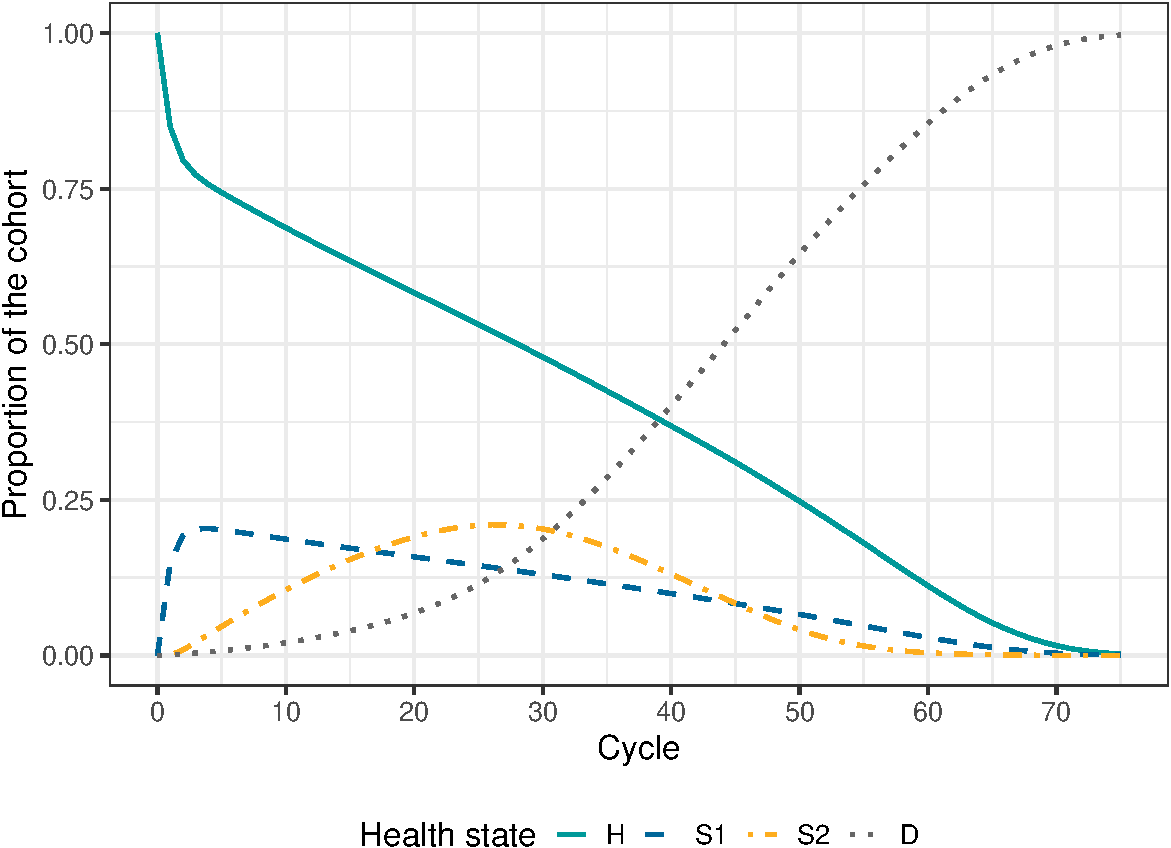
\includegraphics{figs/Sick-Sicker-Trace-HistDep-1} 

}

\caption{Cohort trace of the age-dependent cSTM accounting for state-residence dependency under strategies SoC and A.}\label{fig:Sick-Sicker-Trace-HistDep}
\end{figure}

\hypertarget{epidemiological-and-economic-measures}{%
\section{Epidemiological and economic measures}\label{epidemiological-and-economic-measures}}

cSTMs can be used to generate different epidemiological and economic outputs. In a CEA, the main outcomes are typically the total discounted expected QALYs and total costs accrued by the cohort over the predefined time horizon. However, epidemiological outcomes can be helpful for complementary analyses, such as calibration and validation. Some common epidemiological outcomes include survival, prevalence, incidence, the average number of events, and lifetime risk of events.\textsuperscript{\protect\hyperlink{ref-Siebert2012c}{16}} We show how to obtain some of these outcomes from the trace and transition probability objects.

\hypertarget{epidemiological-measures}{%
\subsection{Epidemiological measures}\label{epidemiological-measures}}

Here we provide the epidemiological definition of some of these outcomes and how they can be generated from a cSTM using the simulation-time-dependent Sick-Sicker cSTM under SoC. In the GitHub repository, we provide the code to generate these outcomes from the state-residence-dependent cSTM.

\hypertarget{survival-probability}{%
\subsubsection{Survival probability}\label{survival-probability}}

The survival probability, \(S(t)\), captures the proportion of the cohort remaining alive by cycle \(t\). To estimate \(S(t)\) from the simulated cohort of the simulation-time-dependent Sick-Sicker model, shown in Figure \ref{fig:Sick-Sicker-Surv-AgeDep}, we sum the proportions of the non-death states for all \(n_T\) cycles in \texttt{m\_M\_SoC}.

\begin{Shaded}
\begin{Highlighting}[]
\NormalTok{v\_S\_SoC }\OtherTok{\textless{}{-}} \FunctionTok{rowSums}\NormalTok{(m\_M\_SoC[, }\SpecialCharTok{{-}}\FunctionTok{which}\NormalTok{(v\_names\_states }\SpecialCharTok{==} \StringTok{"D"}\NormalTok{)]) }\CommentTok{\# vector with survival curve}
\end{Highlighting}
\end{Shaded}

\begin{figure}[H]

{\centering 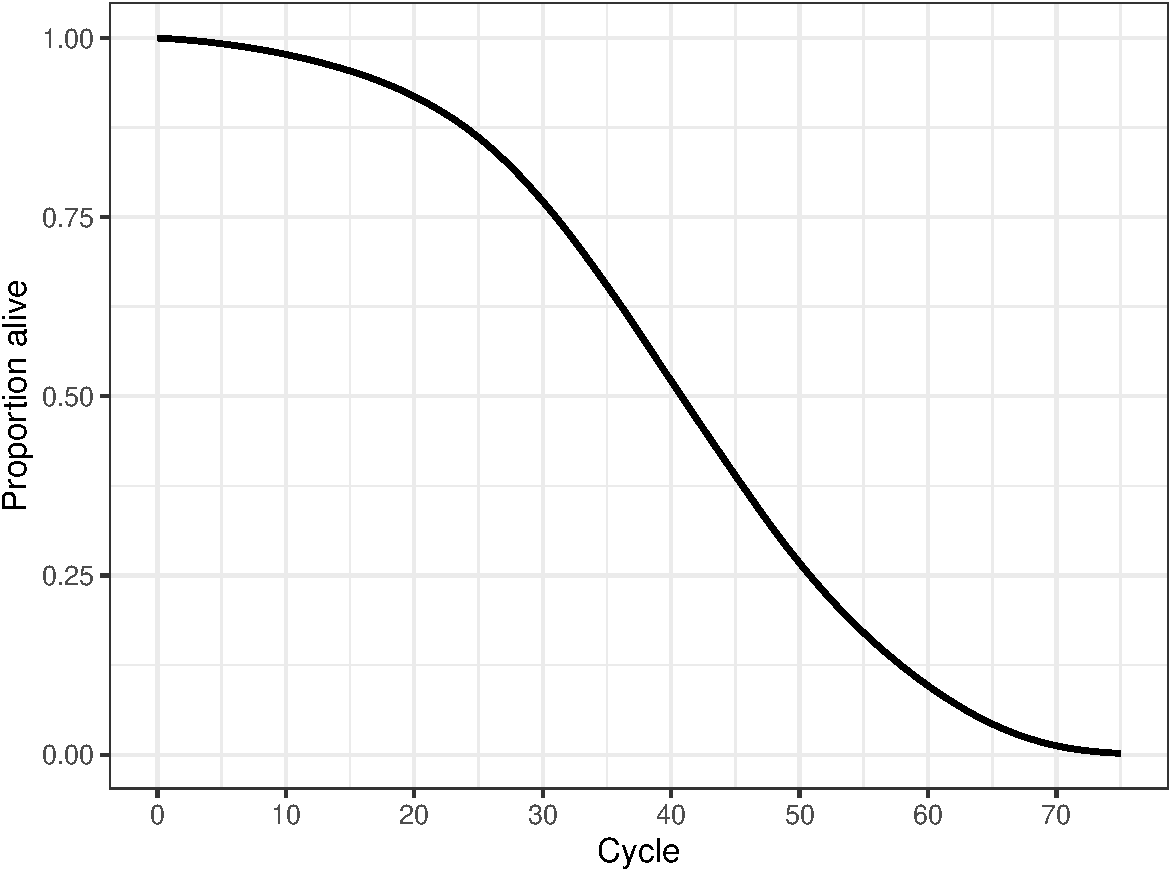
\includegraphics{figs/Sick-Sicker-Surv-AgeDep-1} 

}

\caption{Survival curve of the age-dependent cSTM}\label{fig:Sick-Sicker-Surv-AgeDep}
\end{figure}

\hypertarget{life-expectancy}{%
\subsubsection{Life expectancy}\label{life-expectancy}}

Life expectancy (LE) refers to the expected number of time units remaining to be alive.\textsuperscript{\protect\hyperlink{ref-Lee2003a}{17}} In continuous-time, LE is the area under the entire survival curve.\textsuperscript{\protect\hyperlink{ref-Klein2003}{18}}

\[
LE = \int_{t=0}^{\infty}{S(t) dt}.
\]

In discrete-time using cSTMs, we often calculate restricted LE over a fixed time horizon (e.g., \(n_T\)) at which most of the cohort has transitioned to the Dead state and is defined as

\[
  LE = \sum_{t=0}^{n_T}{S(t)}.
\]

In the simulation-time-dependent Sick-Sicker model, where we simulated a cohort over \(n_T\)= 75 cycles, life expectancy \texttt{le\_SoC} is 41.2 cycles, which is calculated as

\begin{Shaded}
\begin{Highlighting}[]
\NormalTok{le\_SoC }\OtherTok{\textless{}{-}} \FunctionTok{sum}\NormalTok{(v\_S\_SoC) }\CommentTok{\# life expectancy}
\end{Highlighting}
\end{Shaded}

Note that this equation expresses LE in the units of \(t\). We use an annual cycle length; thus, the resulting LE will be in years. Analysts can also use other cycle lengths (e.g., monthly or daily), but the LE must be correctly converted to the desired unit if different than the cycle length units.

\hypertarget{prevalence}{%
\subsubsection{Prevalence}\label{prevalence}}

Prevalence is defined as the proportion of the population or cohort with a specific condition (or being in a particular health state) among those alive.\textsuperscript{\protect\hyperlink{ref-Rothman2008h}{19}} To calculate the prevalence of S1 at cycle \(t\), \(\text{prev}(t)_i\), we compute the ratio between the proportion of the cohort in S1 and the proportion alive at that cycle.\textsuperscript{\protect\hyperlink{ref-Keiding1991}{20}} The proportion of the cohort alive is given by the survival probability \(S(t)\) defined above. The individual prevalence of the S1 and S2 health states and the overall prevalence of sick individuals (i.e., S1 + S2) of the age-dependent Sick-Sicker cSTM at each cycle \(t\) is computed as follows and are shown in Figure \ref{fig:Sick-Sicker-Prev-AgeDep}.

\begin{Shaded}
\begin{Highlighting}[]
\NormalTok{v\_prev\_S1\_SoC   }\OtherTok{\textless{}{-}}\NormalTok{ m\_M\_SoC[, }\StringTok{"S1"}\NormalTok{] }\SpecialCharTok{/}\NormalTok{ v\_S\_SoC          }\CommentTok{\# vector with prevalence of Sick}
\NormalTok{v\_prev\_S2\_SoC   }\OtherTok{\textless{}{-}}\NormalTok{ m\_M\_SoC[, }\StringTok{"S2"}\NormalTok{] }\SpecialCharTok{/}\NormalTok{ v\_S\_SoC          }\CommentTok{\# vector with prevalence of Sicker}
\NormalTok{v\_prev\_S1S2\_SoC }\OtherTok{\textless{}{-}} \FunctionTok{rowSums}\NormalTok{(m\_M\_SoC[, }\FunctionTok{c}\NormalTok{(}\StringTok{"S1"}\NormalTok{, }\StringTok{"S2"}\NormalTok{)])}\SpecialCharTok{/}\NormalTok{v\_S\_SoC }\CommentTok{\# prevalence of Sick and Sicker}
\end{Highlighting}
\end{Shaded}

\begin{figure}[H]

{\centering 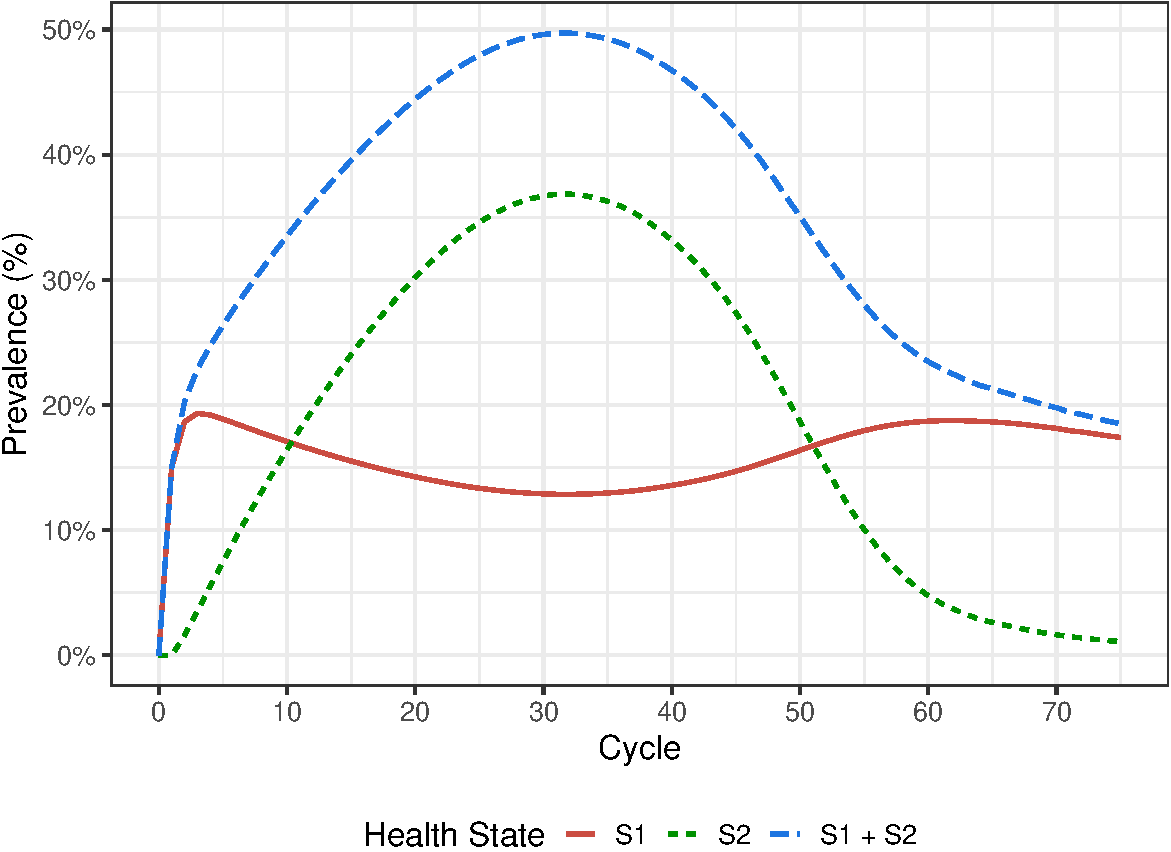
\includegraphics{figs/Sick-Sicker-Prev-AgeDep-1} 

}

\caption{Prevalence of sick states in simulation-time-dependent cSTM}\label{fig:Sick-Sicker-Prev-AgeDep}
\end{figure}

\hypertarget{economic-measures}{%
\subsection{Economic measures}\label{economic-measures}}

In CEA, we can calculate economic outcomes by using either state or transition rewards. A ``state reward'' refers to a value (e.g., cost, utility) assigned to individuals for remaining in a given health state for one cycle. A ``transition reward'' refers to the increase or decrease in either costs or utilities of transitioning from one health state to another, which may be associated with a one-time cost or utility impact. In the accompanying tutorial, we describe how to incorporate state rewards in CEA in detail.\textsuperscript{\protect\hyperlink{ref-Alarid-Escudero2021a}{7}} Here, we describe and illustrate how to implement both state and transition rewards together using a transition array.

\hypertarget{state-rewards}{%
\subsubsection{State rewards}\label{state-rewards}}

As shown in the introductory tutorial, to add state rewards to the Sick-Sicker model, we first create a vector of utilities and costs for each of the four strategies considered. The vectors of utilities and costs, \texttt{v\_u\_SoC} and \texttt{v\_c\_SoC}, respectively, contain the utilities and costs corresponding to being in each of the four health states under SoC, shown in Table \ref{tab:param-table}.

\begin{Shaded}
\begin{Highlighting}[]
\CommentTok{\# Vector of state utilities under SoC}
\NormalTok{v\_u\_SoC }\OtherTok{\textless{}{-}} \FunctionTok{c}\NormalTok{(}\AttributeTok{H =}\NormalTok{ u\_H, }\AttributeTok{S1 =}\NormalTok{ u\_S1, }\AttributeTok{S2 =}\NormalTok{ u\_S2, }\AttributeTok{D =}\NormalTok{ u\_D)}
\CommentTok{\# Vector of state costs under SoC}
\NormalTok{v\_c\_SoC }\OtherTok{\textless{}{-}} \FunctionTok{c}\NormalTok{(}\AttributeTok{H =}\NormalTok{ c\_H, }\AttributeTok{S1 =}\NormalTok{ c\_S1, }\AttributeTok{S2 =}\NormalTok{ c\_S2, }\AttributeTok{D =}\NormalTok{ c\_D)}
\end{Highlighting}
\end{Shaded}

We account for the benefits and costs of both treatments individually and their combination to create the state-reward vectors under treatments A and B (strategies A and B, respectively) and when applied jointly (strategy AB). Only treatment A affects QoL, so we create a vector of utilities for strategy A, \texttt{v\_u\_strA}, where we substitute the utility of being in S1 under SoC, \texttt{u\_S1}, with the utility associated with the benefit of treatment A in being in that state, \texttt{u\_trtA}. Treatment B does not affect QoL, so the vector of utilities for strategy B, \texttt{v\_u\_strB}, is the same as SoC's vector. However, when both treatments A and B are applied jointly (strategy AB), the resulting vector of utilities \texttt{v\_u\_strAB} equals that of strategy A.

\begin{Shaded}
\begin{Highlighting}[]
\CommentTok{\# Vector of state utilities for strategy A}
\NormalTok{v\_u\_strA }\OtherTok{\textless{}{-}} \FunctionTok{c}\NormalTok{(}\AttributeTok{H =}\NormalTok{ u\_H, }\AttributeTok{S1 =}\NormalTok{ u\_trtA, }\AttributeTok{S2 =}\NormalTok{ u\_S2, }\AttributeTok{D =}\NormalTok{ u\_D)}
\CommentTok{\# Vector of state utilities for strategy B}
\NormalTok{v\_u\_strB }\OtherTok{\textless{}{-}}\NormalTok{ v\_u\_SoC}
\CommentTok{\# Vector of state utilities for strategy AB}
\NormalTok{v\_u\_strAB }\OtherTok{\textless{}{-}}\NormalTok{ v\_u\_strA}
\end{Highlighting}
\end{Shaded}

Both treatments A and B incur a cost. To create the vector of state costs for strategy A, \texttt{v\_c\_strA}, we add the cost of treatment A, \texttt{c\_trtA}, to S1 and S2 state costs. Similarly, when constructing the vector of state costs for strategy B, \texttt{v\_c\_strB}, we add the cost of treatment B, \texttt{c\_trtB}, to S1 and S2 state costs. Finally, for the vector of state costs for strategy AB, \texttt{v\_c\_strAB}, we add both treatment costs to the state costs of S1 and S2.

\begin{Shaded}
\begin{Highlighting}[]
\CommentTok{\# Vector of state costs for strategy A}
\NormalTok{v\_c\_strA }\OtherTok{\textless{}{-}} \FunctionTok{c}\NormalTok{(}\AttributeTok{H  =}\NormalTok{ c\_H, }
              \AttributeTok{S1 =}\NormalTok{ c\_S1 }\SpecialCharTok{+}\NormalTok{ c\_trtA, }
              \AttributeTok{S2 =}\NormalTok{ c\_S2 }\SpecialCharTok{+}\NormalTok{ c\_trtA, }
              \AttributeTok{D  =}\NormalTok{ c\_D)}
\CommentTok{\# Vector of state costs for strategy B}
\NormalTok{v\_c\_strB }\OtherTok{\textless{}{-}} \FunctionTok{c}\NormalTok{(}\AttributeTok{H  =}\NormalTok{ c\_H, }
              \AttributeTok{S1 =}\NormalTok{ c\_S1 }\SpecialCharTok{+}\NormalTok{ c\_trtB, }
              \AttributeTok{S2 =}\NormalTok{ c\_S2 }\SpecialCharTok{+}\NormalTok{ c\_trtB, }
              \AttributeTok{D  =}\NormalTok{ c\_D)}
\CommentTok{\# Vector of state costs for strategy AB}
\NormalTok{v\_c\_strAB }\OtherTok{\textless{}{-}} \FunctionTok{c}\NormalTok{(}\AttributeTok{H  =}\NormalTok{ c\_H, }
               \AttributeTok{S1 =}\NormalTok{ c\_S1 }\SpecialCharTok{+}\NormalTok{ (c\_trtA }\SpecialCharTok{+}\NormalTok{ c\_trtB), }
               \AttributeTok{S2 =}\NormalTok{ c\_S2 }\SpecialCharTok{+}\NormalTok{ (c\_trtA }\SpecialCharTok{+}\NormalTok{ c\_trtB), }
               \AttributeTok{D  =}\NormalTok{ c\_D)}
\end{Highlighting}
\end{Shaded}

\hypertarget{transition-rewards}{%
\subsubsection{Transition rewards}\label{transition-rewards}}

In the Sick-Sicker model, we previously mentioned that dying (i.e., transitioning to the Dead state) incurs a one-time cost of \$2,000 that reflects the acute care that might be received immediately preceding death. This one-time cost could include emergency services, hospitalization, other healthcare utilization to address the ultimately fatal health complication, or funeral costs. We also have a utility decrement and a cost increment on the transition from H to S1. These changes in utility and costs represent the short-term impact of the acute events of becoming sick, such as hospitalization, stabilization, and so on, whereas the state rewards of S1 described in the previous section reflect the cost and utility of being chronically sick.

Incorporating transition rewards requires keeping track of the proportion of the cohort that transitions between health states in each cycle while capturing what the states of origin and destination are. The cohort trace, \(M\), does not capture this information. However, obtaining this information is relatively straightforward in a cSTM and described in detail by Krijkamp et al.~(2020).\textsuperscript{\protect\hyperlink{ref-Krijkamp2019}{9}} Briefly, this approach involves changing the core computation in a traditional cSTM, from \(m_t P_t\) to \(\text{diag}(m_t) P_t\). This simple change allows us to compute the proportion of the cohort that transitions between the states of origin and destination in cycle \(t\). The result is no longer a cohort trace matrix, but rather a three-dimensional array that we refer to as a transition-dynamics array (\(\mathbf{A}\)) with dimensions \(n_S \times n_S \times [n_T+1]\). The \(t-\)th slice of \(\mathbf{A}\), \(A_t\), is a matrix that stores the proportion of the population that transition between states of origin and destination between cycles \(t-1\) and \(t\). Similarly, we define the transition rewards by the states of origin and destination.

To account for both state and transition rewards, we create a \emph{matrix} of rewards \(R_t\) of dimensions \(n_S \times n_S\). The off-diagonal entries of \(R_t\) store the transition rewards, and the diagonal of \(R_t\) stores the state rewards for cycle \(t\) and assumes that rewards occur at the beginning of the cycle.\textsuperscript{\protect\hyperlink{ref-Krijkamp2019}{9}} Finally, we multiply this matrix by \(A_t\), the \(t\)-th slice of \(A\), apply discounting, within-cycle correction, and compute the overall reward for each strategy outcome. Below, we illustrate these concepts in R.

To compute \(\mathbf{A}\) for the simulation-time-dependent Sick-Sicker model under SoC, we initialize a three-dimensional array \texttt{a\_A\_SoC} of dimensions \(n_S \times n_S \times [n_T+1]\) and set the diagonal of the first slice to the initial state vector \texttt{v\_s\_init}. Next, we create a three-dimensional array for each of the strategies as a copy of the array under SoC.

\begin{Shaded}
\begin{Highlighting}[]
\CommentTok{\# Initialize transition{-}dynamics array under SoC}
\NormalTok{a\_A\_SoC }\OtherTok{\textless{}{-}} \FunctionTok{array}\NormalTok{(}\DecValTok{0}\NormalTok{,}
             \AttributeTok{dim =} \FunctionTok{c}\NormalTok{(n\_states, n\_states, (n\_cycles }\SpecialCharTok{+} \DecValTok{1}\NormalTok{)),}
             \AttributeTok{dimnames =} \FunctionTok{list}\NormalTok{(v\_names\_states, v\_names\_states, }\DecValTok{0}\SpecialCharTok{:}\NormalTok{n\_cycles))}
\CommentTok{\# Set first slice to the initial state vector in its diagonal}
\FunctionTok{diag}\NormalTok{(a\_A\_SoC[, , }\DecValTok{1}\NormalTok{]) }\OtherTok{\textless{}{-}}\NormalTok{ v\_s\_init}
\CommentTok{\# Initialize transition{-}dynamics array for strategies A, B, and AB}
\CommentTok{\# Structure and initial states are the same as for SoC}
\NormalTok{a\_A\_strA  }\OtherTok{\textless{}{-}}\NormalTok{ a\_A\_SoC}
\NormalTok{a\_A\_strB  }\OtherTok{\textless{}{-}}\NormalTok{ a\_A\_SoC}
\NormalTok{a\_A\_strAB }\OtherTok{\textless{}{-}}\NormalTok{ a\_A\_SoC}
\end{Highlighting}
\end{Shaded}

We then compute a matrix multiplication between a diagonal matrix of each of the \(t\)-th rows of the cohort trace matrix under SoC and treatment B, denoted as \texttt{diag(m\_M\_SoC{[}t,\ {]})} and \texttt{diag(m\_M\_strB{[}t,\ {]})}, by the \(t\)-th matrix of the array of transition matrices, \texttt{a\_P\_SoC{[},\ ,\ t{]}} and \texttt{a\_P\_strB{[},\ ,\ t{]}}, respectively, over all \(n_T\) cycles.

\begin{Shaded}
\begin{Highlighting}[]
\CommentTok{\# Iterative solution to produce the transition{-}dynamics array}
\ControlFlowTok{for}\NormalTok{ (t }\ControlFlowTok{in} \DecValTok{1}\SpecialCharTok{:}\NormalTok{n\_cycles)\{}
  \CommentTok{\# For SoC}
\NormalTok{  a\_A\_SoC[, , t }\SpecialCharTok{+} \DecValTok{1}\NormalTok{] }\OtherTok{\textless{}{-}} \FunctionTok{diag}\NormalTok{(m\_M\_SoC[t, ]) }\SpecialCharTok{\%*\%}\NormalTok{ a\_P\_SoC[, , t]}
  \CommentTok{\# For strategy A}
\NormalTok{  a\_A\_strA[, , t }\SpecialCharTok{+} \DecValTok{1}\NormalTok{] }\OtherTok{\textless{}{-}} \FunctionTok{diag}\NormalTok{(m\_M\_strA[t, ]) }\SpecialCharTok{\%*\%}\NormalTok{ a\_P\_strA[, , t]}
  \CommentTok{\# For strategy B}
\NormalTok{  a\_A\_strB[, , t }\SpecialCharTok{+} \DecValTok{1}\NormalTok{] }\OtherTok{\textless{}{-}} \FunctionTok{diag}\NormalTok{(m\_M\_strB[t, ]) }\SpecialCharTok{\%*\%}\NormalTok{ a\_P\_strB[, , t]}
  \CommentTok{\# For strategy AB}
\NormalTok{  a\_A\_strAB[, , t }\SpecialCharTok{+} \DecValTok{1}\NormalTok{] }\OtherTok{\textless{}{-}} \FunctionTok{diag}\NormalTok{(m\_M\_strAB[t, ]) }\SpecialCharTok{\%*\%}\NormalTok{ a\_P\_strAB[, , t]}
\NormalTok{\}}
\end{Highlighting}
\end{Shaded}

To create the arrays of rewards for costs and utilities for the simulation-time-dependent Sick-Sicker cSTM, we create strategy-specific three-dimensional arrays of rewards and fill each of their rows across the third dimension with the vector of state rewards.

\begin{Shaded}
\begin{Highlighting}[]
\CommentTok{\# Arrays of state and transition rewards}
\CommentTok{\# Utilities under SoC}
\NormalTok{a\_R\_u\_SoC }\OtherTok{\textless{}{-}} \FunctionTok{array}\NormalTok{(}\FunctionTok{matrix}\NormalTok{(v\_u\_SoC, }\AttributeTok{nrow =}\NormalTok{ n\_states, }\AttributeTok{ncol =}\NormalTok{ n\_states, }\AttributeTok{byrow =}\NormalTok{ T), }
                  \AttributeTok{dim =} \FunctionTok{c}\NormalTok{(n\_states, n\_states, n\_cycles }\SpecialCharTok{+} \DecValTok{1}\NormalTok{),}
                  \AttributeTok{dimnames =} \FunctionTok{list}\NormalTok{(v\_names\_states, v\_names\_states, }\DecValTok{0}\SpecialCharTok{:}\NormalTok{n\_cycles))}
\CommentTok{\# Costs under SoC}
\NormalTok{a\_R\_c\_SoC }\OtherTok{\textless{}{-}} \FunctionTok{array}\NormalTok{(}\FunctionTok{matrix}\NormalTok{(v\_c\_SoC, }\AttributeTok{nrow =}\NormalTok{ n\_states, }\AttributeTok{ncol =}\NormalTok{ n\_states, }\AttributeTok{byrow =}\NormalTok{ T), }
                  \AttributeTok{dim =} \FunctionTok{c}\NormalTok{(n\_states, n\_states, n\_cycles }\SpecialCharTok{+} \DecValTok{1}\NormalTok{),}
                  \AttributeTok{dimnames =} \FunctionTok{list}\NormalTok{(v\_names\_states, v\_names\_states, }\DecValTok{0}\SpecialCharTok{:}\NormalTok{n\_cycles))}
\CommentTok{\# Utilities under Strategy A}
\NormalTok{a\_R\_u\_strA }\OtherTok{\textless{}{-}}  \FunctionTok{array}\NormalTok{(}\FunctionTok{matrix}\NormalTok{(v\_u\_strA, }\AttributeTok{nrow =}\NormalTok{ n\_states, }\AttributeTok{ncol =}\NormalTok{ n\_states, }\AttributeTok{byrow =}\NormalTok{ T), }
                  \AttributeTok{dim =} \FunctionTok{c}\NormalTok{(n\_states, n\_states, n\_cycles }\SpecialCharTok{+} \DecValTok{1}\NormalTok{),}
                  \AttributeTok{dimnames =} \FunctionTok{list}\NormalTok{(v\_names\_states, v\_names\_states, }\DecValTok{0}\SpecialCharTok{:}\NormalTok{n\_cycles))}
\CommentTok{\# Costs under Strategy A}
\NormalTok{a\_R\_c\_strA }\OtherTok{\textless{}{-}} \FunctionTok{array}\NormalTok{(}\FunctionTok{matrix}\NormalTok{(v\_c\_strA, }\AttributeTok{nrow =}\NormalTok{ n\_states, }\AttributeTok{ncol =}\NormalTok{ n\_states, }\AttributeTok{byrow =}\NormalTok{ T), }
                  \AttributeTok{dim =} \FunctionTok{c}\NormalTok{(n\_states, n\_states, n\_cycles }\SpecialCharTok{+} \DecValTok{1}\NormalTok{),}
                  \AttributeTok{dimnames =} \FunctionTok{list}\NormalTok{(v\_names\_states, v\_names\_states, }\DecValTok{0}\SpecialCharTok{:}\NormalTok{n\_cycles))}
\CommentTok{\# Utilities under Strategy B}
\NormalTok{a\_R\_u\_strB }\OtherTok{\textless{}{-}}  \FunctionTok{array}\NormalTok{(}\FunctionTok{matrix}\NormalTok{(v\_u\_strB, }\AttributeTok{nrow =}\NormalTok{ n\_states, }\AttributeTok{ncol =}\NormalTok{ n\_states, }\AttributeTok{byrow =}\NormalTok{ T), }
                  \AttributeTok{dim =} \FunctionTok{c}\NormalTok{(n\_states, n\_states, n\_cycles }\SpecialCharTok{+} \DecValTok{1}\NormalTok{),}
                  \AttributeTok{dimnames =} \FunctionTok{list}\NormalTok{(v\_names\_states, v\_names\_states, }\DecValTok{0}\SpecialCharTok{:}\NormalTok{n\_cycles))}
\CommentTok{\# Costs under Strategy B}
\NormalTok{a\_R\_c\_strB }\OtherTok{\textless{}{-}} \FunctionTok{array}\NormalTok{(}\FunctionTok{matrix}\NormalTok{(v\_c\_strB, }\AttributeTok{nrow =}\NormalTok{ n\_states, }\AttributeTok{ncol =}\NormalTok{ n\_states, }\AttributeTok{byrow =}\NormalTok{ T), }
                  \AttributeTok{dim =} \FunctionTok{c}\NormalTok{(n\_states, n\_states, n\_cycles }\SpecialCharTok{+} \DecValTok{1}\NormalTok{),}
                  \AttributeTok{dimnames =} \FunctionTok{list}\NormalTok{(v\_names\_states, v\_names\_states, }\DecValTok{0}\SpecialCharTok{:}\NormalTok{n\_cycles))}
\CommentTok{\# Utilities under Strategy AB}
\NormalTok{a\_R\_u\_strAB }\OtherTok{\textless{}{-}}  \FunctionTok{array}\NormalTok{(}\FunctionTok{matrix}\NormalTok{(v\_u\_strAB, }\AttributeTok{nrow =}\NormalTok{ n\_states, }\AttributeTok{ncol =}\NormalTok{ n\_states, }\AttributeTok{byrow =}\NormalTok{ T), }
                  \AttributeTok{dim =} \FunctionTok{c}\NormalTok{(n\_states, n\_states, n\_cycles }\SpecialCharTok{+} \DecValTok{1}\NormalTok{),}
                  \AttributeTok{dimnames =} \FunctionTok{list}\NormalTok{(v\_names\_states, v\_names\_states, }\DecValTok{0}\SpecialCharTok{:}\NormalTok{n\_cycles))}
\CommentTok{\# Costs under Strategy AB}
\NormalTok{a\_R\_c\_strAB }\OtherTok{\textless{}{-}} \FunctionTok{array}\NormalTok{(}\FunctionTok{matrix}\NormalTok{(v\_c\_strAB, }\AttributeTok{nrow =}\NormalTok{ n\_states, }\AttributeTok{ncol =}\NormalTok{ n\_states, }\AttributeTok{byrow =}\NormalTok{ T), }
                  \AttributeTok{dim =} \FunctionTok{c}\NormalTok{(n\_states, n\_states, n\_cycles }\SpecialCharTok{+} \DecValTok{1}\NormalTok{),}
                  \AttributeTok{dimnames =} \FunctionTok{list}\NormalTok{(v\_names\_states, v\_names\_states, }\DecValTok{0}\SpecialCharTok{:}\NormalTok{n\_cycles))}
\end{Highlighting}
\end{Shaded}

To account for the transition rewards, we either add or subtract them in the corresponding location of the reward matrix representing the transitions of interest. Thus, for example, to account for the disutility of transitioning from H to S1 under strategy A, we subtract the disutility to the entry of the array of rewards corresponding to the transition from H to S1 across all cycles.

\begin{Shaded}
\begin{Highlighting}[]
\CommentTok{\# Add disutility due to transition from Healthy to Sick}
\NormalTok{a\_R\_u\_strA[}\StringTok{"H"}\NormalTok{, }\StringTok{"S1"}\NormalTok{, ] }\OtherTok{\textless{}{-}}\NormalTok{ a\_R\_u\_strA[}\StringTok{"H"}\NormalTok{, }\StringTok{"S1"}\NormalTok{, ] }\SpecialCharTok{{-}}\NormalTok{ du\_HS1}
\end{Highlighting}
\end{Shaded}

In a similar approach, we add the costs of transitioning from H to S1 and the cost of dying under strategy A.

\begin{Shaded}
\begin{Highlighting}[]
\CommentTok{\# Add transition cost due to transition from Healthy to Sick}
\NormalTok{a\_R\_c\_strA[}\StringTok{"H"}\NormalTok{, }\StringTok{"S1"}\NormalTok{, ] }\OtherTok{\textless{}{-}}\NormalTok{ a\_R\_c\_strA[}\StringTok{"H"}\NormalTok{, }\StringTok{"S1"}\NormalTok{, ] }\SpecialCharTok{+}\NormalTok{ ic\_HS1}
\CommentTok{\# Add transition cost of dying from all non{-}dead states}
\NormalTok{a\_R\_c\_strA[}\SpecialCharTok{{-}}\NormalTok{n\_states, }\StringTok{"D"}\NormalTok{, ] }\OtherTok{\textless{}{-}}\NormalTok{ a\_R\_c\_strA[}\SpecialCharTok{{-}}\NormalTok{n\_states, }\StringTok{"D"}\NormalTok{, ] }\SpecialCharTok{+}\NormalTok{ ic\_D}
\NormalTok{a\_R\_c\_strA[, , }\DecValTok{1}\NormalTok{]}
\end{Highlighting}
\end{Shaded}

\begin{verbatim}
##       H    S1    S2    D
## H  2000 17000 27000 2000
## S1 2000 16000 27000 2000
## S2 2000 16000 27000 2000
## D  2000 16000 27000    0
\end{verbatim}

Below, we show how to add the transition rewards to the reward matrices under SoC and strategies B and AB.

\begin{Shaded}
\begin{Highlighting}[]
\DocumentationTok{\#\# SoC}
\CommentTok{\# Add disutility due to transition from H to S1}
\NormalTok{a\_R\_u\_SoC[}\StringTok{"H"}\NormalTok{, }\StringTok{"S1"}\NormalTok{, ] }\OtherTok{\textless{}{-}}\NormalTok{ a\_R\_u\_SoC[}\StringTok{"H"}\NormalTok{, }\StringTok{"S1"}\NormalTok{, ] }\SpecialCharTok{{-}}\NormalTok{ du\_HS1}
\CommentTok{\# Add transition cost due to transition from H to S1}
\NormalTok{a\_R\_c\_SoC[}\StringTok{"H"}\NormalTok{, }\StringTok{"S1"}\NormalTok{, ] }\OtherTok{\textless{}{-}}\NormalTok{ a\_R\_c\_SoC[}\StringTok{"H"}\NormalTok{, }\StringTok{"S1"}\NormalTok{, ] }\SpecialCharTok{+}\NormalTok{ ic\_HS1}
\CommentTok{\# Add transition cost of dying from all non{-}dead states}
\NormalTok{a\_R\_c\_SoC[}\SpecialCharTok{{-}}\NormalTok{n\_states, }\StringTok{"D"}\NormalTok{, ] }\OtherTok{\textless{}{-}}\NormalTok{ a\_R\_c\_SoC[}\SpecialCharTok{{-}}\NormalTok{n\_states, }\StringTok{"D"}\NormalTok{, ] }\SpecialCharTok{+}\NormalTok{ ic\_D}

\DocumentationTok{\#\# Strategy B}
\CommentTok{\# Add disutility due to transition from Healthy to Sick}
\NormalTok{a\_R\_u\_strB[}\StringTok{"H"}\NormalTok{, }\StringTok{"S1"}\NormalTok{, ] }\OtherTok{\textless{}{-}}\NormalTok{ a\_R\_u\_strB[}\StringTok{"H"}\NormalTok{, }\StringTok{"S1"}\NormalTok{, ] }\SpecialCharTok{{-}}\NormalTok{ du\_HS1}
\CommentTok{\# Add transition cost due to transition from Healthy to Sick}
\NormalTok{a\_R\_c\_strB[}\StringTok{"H"}\NormalTok{, }\StringTok{"S1"}\NormalTok{, ] }\OtherTok{\textless{}{-}}\NormalTok{ a\_R\_c\_strB[}\StringTok{"H"}\NormalTok{, }\StringTok{"S1"}\NormalTok{, ] }\SpecialCharTok{+}\NormalTok{ ic\_HS1}
\CommentTok{\# Add transition cost of dying from all non{-}dead states}
\NormalTok{a\_R\_c\_strB[}\SpecialCharTok{{-}}\NormalTok{n\_states, }\StringTok{"D"}\NormalTok{, ] }\OtherTok{\textless{}{-}}\NormalTok{ a\_R\_c\_strB[}\SpecialCharTok{{-}}\NormalTok{n\_states, }\StringTok{"D"}\NormalTok{, ] }\SpecialCharTok{+}\NormalTok{ ic\_D}

\DocumentationTok{\#\# Strategy AB}
\CommentTok{\# Add disutility due to transition from Healthy to Sick}
\NormalTok{a\_R\_u\_strAB[}\StringTok{"H"}\NormalTok{, }\StringTok{"S1"}\NormalTok{, ] }\OtherTok{\textless{}{-}}\NormalTok{ a\_R\_u\_strAB[}\StringTok{"H"}\NormalTok{, }\StringTok{"S1"}\NormalTok{, ] }\SpecialCharTok{{-}}\NormalTok{ du\_HS1}
\CommentTok{\# Add transition cost due to transition from Healthy to Sick}
\NormalTok{a\_R\_c\_strAB[}\StringTok{"H"}\NormalTok{, }\StringTok{"S1"}\NormalTok{, ] }\OtherTok{\textless{}{-}}\NormalTok{ a\_R\_c\_strAB[}\StringTok{"H"}\NormalTok{, }\StringTok{"S1"}\NormalTok{, ] }\SpecialCharTok{+}\NormalTok{ ic\_HS1}
\CommentTok{\# Add transition cost of dying from all non{-}dead states}
\NormalTok{a\_R\_c\_strAB[}\SpecialCharTok{{-}}\NormalTok{n\_states, }\StringTok{"D"}\NormalTok{, ] }\OtherTok{\textless{}{-}}\NormalTok{ a\_R\_c\_strAB[}\SpecialCharTok{{-}}\NormalTok{n\_states, }\StringTok{"D"}\NormalTok{, ] }\SpecialCharTok{+}\NormalTok{ ic\_D}
\end{Highlighting}
\end{Shaded}

The state and transition rewards are applied to the model dynamics by element-wise multiplication between \(\mathbf{A}\) and \(\mathbf{R}\), indicated by the \(\odot\) sign, which produces the array of outputs for all \(n_T\) cycles, \(\mathbf{Y}\). Formally,
\begin{equation}
  \mathbf{Y} = \mathbf{A} \odot \mathbf{R}
  \label{eq:array-outputs}
\end{equation}

To obtain \(\mathbf{Y}\) for QALYs and costs for all four strategies, we apply Equation \eqref{eq:array-outputs} by the element-wise multiplication of the transition array \texttt{a\_A\_SoC} by the corresponding array of rewards.

\begin{Shaded}
\begin{Highlighting}[]
\CommentTok{\# For SoC}
\NormalTok{a\_Y\_c\_SoC }\OtherTok{\textless{}{-}}\NormalTok{ a\_A\_SoC }\SpecialCharTok{*}\NormalTok{ a\_R\_c\_SoC}
\NormalTok{a\_Y\_u\_SoC }\OtherTok{\textless{}{-}}\NormalTok{ a\_A\_SoC }\SpecialCharTok{*}\NormalTok{ a\_R\_u\_SoC}
\CommentTok{\# For Strategy A}
\NormalTok{a\_Y\_c\_strA }\OtherTok{\textless{}{-}}\NormalTok{ a\_A\_strA }\SpecialCharTok{*}\NormalTok{ a\_R\_c\_strA}
\NormalTok{a\_Y\_u\_strA }\OtherTok{\textless{}{-}}\NormalTok{ a\_A\_strA }\SpecialCharTok{*}\NormalTok{ a\_R\_u\_strA}
\CommentTok{\# For Strategy B}
\NormalTok{a\_Y\_c\_strB }\OtherTok{\textless{}{-}}\NormalTok{ a\_A\_strB }\SpecialCharTok{*}\NormalTok{ a\_R\_c\_strB}
\NormalTok{a\_Y\_u\_strB }\OtherTok{\textless{}{-}}\NormalTok{ a\_A\_strB }\SpecialCharTok{*}\NormalTok{ a\_R\_u\_strB}
\CommentTok{\# For Strategy AB}
\NormalTok{a\_Y\_c\_strAB }\OtherTok{\textless{}{-}}\NormalTok{ a\_A\_strAB }\SpecialCharTok{*}\NormalTok{ a\_R\_c\_strAB}
\NormalTok{a\_Y\_u\_strAB }\OtherTok{\textless{}{-}}\NormalTok{ a\_A\_strAB }\SpecialCharTok{*}\NormalTok{ a\_R\_u\_strAB}
\end{Highlighting}
\end{Shaded}

The total rewards for each health state at cycle \(t\), \(\mathbf{y}_t\), is obtained by summing the rewards across all \(j = 1,\ldots, n_S\) health states for all \(n_T\) cycles.
\begin{equation}
  \mathbf{y}_t = \mathbf{1}^T Y_t = \left[\sum_{i=1}^{n_S}{Y_{[i,1,t]}}, \sum_{i=1}^{n_S}{Y_{[i,2,t]}}, \dots , \sum_{i=1}^{n_S}{Y_{[i,n_S,t]}}\right].
  \label{eq:exp-rewd-trans}
\end{equation}

To obtain the expected costs and QALYs per cycle for each strategy, \(\mathbf{y}\), we apply Equation \eqref{eq:exp-rewd-trans} again across all the matrices of the third dimension of \(\mathbf{Y}\) for all the outcomes.

\begin{Shaded}
\begin{Highlighting}[]
\CommentTok{\# Vectors of rewards}
\CommentTok{\# QALYs under SoC}
\NormalTok{v\_qaly\_SoC }\OtherTok{\textless{}{-}} \FunctionTok{rowSums}\NormalTok{(}\FunctionTok{t}\NormalTok{(}\FunctionTok{colSums}\NormalTok{(a\_Y\_u\_SoC)))}
\CommentTok{\# Costs under SoC}
\NormalTok{v\_cost\_SoC }\OtherTok{\textless{}{-}} \FunctionTok{rowSums}\NormalTok{(}\FunctionTok{t}\NormalTok{(}\FunctionTok{colSums}\NormalTok{(a\_Y\_c\_SoC)))}
\CommentTok{\# QALYs under Strategy A}
\NormalTok{v\_qaly\_strA }\OtherTok{\textless{}{-}} \FunctionTok{rowSums}\NormalTok{(}\FunctionTok{t}\NormalTok{(}\FunctionTok{colSums}\NormalTok{(a\_Y\_u\_strA)))}
\CommentTok{\# Costs under Strategy A}
\NormalTok{v\_cost\_strA }\OtherTok{\textless{}{-}} \FunctionTok{rowSums}\NormalTok{(}\FunctionTok{t}\NormalTok{(}\FunctionTok{colSums}\NormalTok{(a\_Y\_c\_strA)))}
\CommentTok{\# QALYs under Strategy B}
\NormalTok{v\_qaly\_strB }\OtherTok{\textless{}{-}} \FunctionTok{rowSums}\NormalTok{(}\FunctionTok{t}\NormalTok{(}\FunctionTok{colSums}\NormalTok{(a\_Y\_u\_strB)))}
\CommentTok{\# Costs under Strategy B}
\NormalTok{v\_cost\_strB }\OtherTok{\textless{}{-}} \FunctionTok{rowSums}\NormalTok{(}\FunctionTok{t}\NormalTok{(}\FunctionTok{colSums}\NormalTok{(a\_Y\_c\_strB)))}
\CommentTok{\# QALYs under Strategy AB}
\NormalTok{v\_qaly\_strAB }\OtherTok{\textless{}{-}} \FunctionTok{rowSums}\NormalTok{(}\FunctionTok{t}\NormalTok{(}\FunctionTok{colSums}\NormalTok{(a\_Y\_u\_strAB)))}
\CommentTok{\# Costs under Strategy AB}
\NormalTok{v\_cost\_strAB }\OtherTok{\textless{}{-}} \FunctionTok{rowSums}\NormalTok{(}\FunctionTok{t}\NormalTok{(}\FunctionTok{colSums}\NormalTok{(a\_Y\_c\_strAB)))}
\end{Highlighting}
\end{Shaded}

\hypertarget{within-cycle-correction-and-discounting-future-rewards}{%
\subsubsection{Within-cycle correction and discounting future rewards}\label{within-cycle-correction-and-discounting-future-rewards}}

Following the accompanying introductory cSTM tutorial,\textsuperscript{\protect\hyperlink{ref-Alarid-Escudero2021a}{7}} here we use Simpson's 1/3rd rule for within-cycle correction (WCC),\textsuperscript{\protect\hyperlink{ref-Elbasha2016a}{22}} and use exponential discounting for costs and QALYs. In our example, the WCC vector, \(\mathbf{wcc}\), is the same for both costs and QALYs; thus, only one vector, \texttt{v\_wcc}, is required.

\begin{Shaded}
\begin{Highlighting}[]
\DocumentationTok{\#\# Vector with cycles}
\NormalTok{v\_cycles }\OtherTok{\textless{}{-}} \FunctionTok{seq}\NormalTok{(}\DecValTok{1}\NormalTok{, n\_cycles}\SpecialCharTok{+}\DecValTok{1}\NormalTok{)}
\DocumentationTok{\#\# Generate 2/3 and 4/3 multipliers for even and odd entries, respectively}
\NormalTok{v\_wcc }\OtherTok{\textless{}{-}}\NormalTok{ ((v\_cycles }\SpecialCharTok{\%\%} \DecValTok{2}\NormalTok{)}\SpecialCharTok{==}\DecValTok{0}\NormalTok{)}\SpecialCharTok{*}\NormalTok{(}\DecValTok{2}\SpecialCharTok{/}\DecValTok{3}\NormalTok{) }\SpecialCharTok{+}\NormalTok{ ((v\_cycles }\SpecialCharTok{\%\%} \DecValTok{2}\NormalTok{)}\SpecialCharTok{!=}\DecValTok{0}\NormalTok{)}\SpecialCharTok{*}\NormalTok{(}\DecValTok{4}\SpecialCharTok{/}\DecValTok{3}\NormalTok{)}
\DocumentationTok{\#\# Substitute 1/3 in first and last entries}
\NormalTok{v\_wcc[}\DecValTok{1}\NormalTok{] }\OtherTok{\textless{}{-}}\NormalTok{ v\_wcc[n\_cycles }\SpecialCharTok{+} \DecValTok{1}\NormalTok{] }\OtherTok{\textless{}{-}} \DecValTok{1}\SpecialCharTok{/}\DecValTok{3}
\end{Highlighting}
\end{Shaded}

The discount vectors, \(\mathbf{d}\), for costs and QALYs for the Sick-Sicker model, \texttt{v\_dwc} and \texttt{v\_dwe}, respectively, are

\begin{Shaded}
\begin{Highlighting}[]
\CommentTok{\# Discount weight for effects}
\NormalTok{v\_dwe }\OtherTok{\textless{}{-}} \DecValTok{1} \SpecialCharTok{/}\NormalTok{ ((}\DecValTok{1} \SpecialCharTok{+}\NormalTok{ d\_e) }\SpecialCharTok{\^{}}\NormalTok{ (}\DecValTok{0}\SpecialCharTok{:}\NormalTok{(n\_cycles)))  }
\CommentTok{\# Discount weight for costs }
\NormalTok{v\_dwc }\OtherTok{\textless{}{-}} \DecValTok{1} \SpecialCharTok{/}\NormalTok{ ((}\DecValTok{1} \SpecialCharTok{+}\NormalTok{ d\_c) }\SpecialCharTok{\^{}}\NormalTok{ (}\DecValTok{0}\SpecialCharTok{:}\NormalTok{(n\_cycles)))    }
\end{Highlighting}
\end{Shaded}

To account for both discounting and WCC, we incorporate \(\mathbf{wcc}\) in equation \eqref{eq:tot-exp-disc-rewd-wcc} using an element-wise multiplication with \(\mathbf{d}\), indicated by the \(\odot\) symbol, such that
\begin{equation}
 y = \mathbf{y}^{'} \left(\mathbf{d} \odot \mathbf{wcc}\right).
 \label{eq:tot-exp-disc-rewd-wcc}
\end{equation}

The total expected discounted costs and QALYs under all four strategies accounting for WCC, \(y\), is obtained by applying Equation \eqref{eq:tot-exp-disc-rewd-wcc} to the expected outcomes accounting for transition rewards.

\begin{Shaded}
\begin{Highlighting}[]
\DocumentationTok{\#\#\# For SoC}
\DocumentationTok{\#\# QALYs}
\NormalTok{n\_tot\_qaly\_SoC }\OtherTok{\textless{}{-}} \FunctionTok{t}\NormalTok{(v\_qaly\_SoC) }\SpecialCharTok{\%*\%}\NormalTok{ (v\_dwe }\SpecialCharTok{*}\NormalTok{ v\_wcc)}
\DocumentationTok{\#\# Costs}
\NormalTok{n\_tot\_cost\_SoC }\OtherTok{\textless{}{-}} \FunctionTok{t}\NormalTok{(v\_cost\_SoC) }\SpecialCharTok{\%*\%}\NormalTok{ (v\_dwc }\SpecialCharTok{*}\NormalTok{ v\_wcc)}
\DocumentationTok{\#\#\# For Strategy A}
\DocumentationTok{\#\# QALYs}
\NormalTok{n\_tot\_qaly\_strA }\OtherTok{\textless{}{-}} \FunctionTok{t}\NormalTok{(v\_qaly\_strA) }\SpecialCharTok{\%*\%}\NormalTok{ (v\_dwe }\SpecialCharTok{*}\NormalTok{ v\_wcc)}
\DocumentationTok{\#\# Costs}
\NormalTok{n\_tot\_cost\_strA }\OtherTok{\textless{}{-}} \FunctionTok{t}\NormalTok{(v\_cost\_strA) }\SpecialCharTok{\%*\%}\NormalTok{ (v\_dwc }\SpecialCharTok{*}\NormalTok{ v\_wcc)}
\DocumentationTok{\#\#\# For Strategy B}
\DocumentationTok{\#\# QALYs}
\NormalTok{n\_tot\_qaly\_strB }\OtherTok{\textless{}{-}} \FunctionTok{t}\NormalTok{(v\_qaly\_strB) }\SpecialCharTok{\%*\%}\NormalTok{ (v\_dwe }\SpecialCharTok{*}\NormalTok{ v\_wcc)}
\DocumentationTok{\#\# Costs}
\NormalTok{n\_tot\_cost\_strB }\OtherTok{\textless{}{-}} \FunctionTok{t}\NormalTok{(v\_cost\_strB) }\SpecialCharTok{\%*\%}\NormalTok{ (v\_dwc }\SpecialCharTok{*}\NormalTok{ v\_wcc)}
\DocumentationTok{\#\#\# For Strategy AB}
\DocumentationTok{\#\# QALYs}
\NormalTok{n\_tot\_qaly\_strAB }\OtherTok{\textless{}{-}} \FunctionTok{t}\NormalTok{(v\_qaly\_strAB) }\SpecialCharTok{\%*\%}\NormalTok{ (v\_dwe }\SpecialCharTok{*}\NormalTok{ v\_wcc)}
\DocumentationTok{\#\# Costs}
\NormalTok{n\_tot\_cost\_strAB }\OtherTok{\textless{}{-}} \FunctionTok{t}\NormalTok{(v\_cost\_strAB) }\SpecialCharTok{\%*\%}\NormalTok{ (v\_dwc }\SpecialCharTok{*}\NormalTok{ v\_wcc)}
\end{Highlighting}
\end{Shaded}

The total expected discounted QALYs and costs for the simulation-time-dependent Sick-Sicker model under the four strategies accounting for WCC are shown in Table \ref{tab:Expected-outcomes-table}.

\begin{table}[!h]

\caption{\label{tab:Expected-outcomes-table}Total expected discounted QALYs and costs per average individual in the cohort of the simulation-time-dependent Sick-Sicker model by strategy accounting for within-cycle correction .}
\centering
\begin{tabular}[t]{llc}
\toprule{}
  & Costs & QALYs\\
\midrule{}
Standard of care & \$114,560 & 19.142\\
Strategy A & \$211,911 & 19.840\\
Strategy B & \$194,481 & 20.480\\
Strategy AB & \$282,370 & 21.302\\
\bottomrule{}
\end{tabular}
\end{table}

\hypertarget{incremental-cost-effectiveness-ratios-icers}{%
\section{Incremental cost-effectiveness ratios (ICERs)}\label{incremental-cost-effectiveness-ratios-icers}}

To conduct the cost-effectiveness analysis, we follow the coding approach described in the accompanying introductory cSTM tutorial.\textsuperscript{\protect\hyperlink{ref-Alarid-Escudero2021a}{7}} We combine the total expected discounted costs and QALYs for all four strategies into outcome-specific vectors, \texttt{v\_cost\_str} for costs and \texttt{v\_qaly\_str} for QALYs. We use the R package \texttt{dampack} (\url{https://cran.r-project.org/web/packages/dampack/})\textsuperscript{\protect\hyperlink{ref-Alarid-Escudero2021}{23}} to calculate the incremental costs and effectiveness and the incremental cost-effectiveness ratio (ICER) between non-dominated strategies. The results are returned as the R the data frame \texttt{df\_cea}.

\begin{Shaded}
\begin{Highlighting}[]
\DocumentationTok{\#\#\# Vector of costs}
\NormalTok{v\_cost\_str }\OtherTok{\textless{}{-}} \FunctionTok{c}\NormalTok{(n\_tot\_cost\_SoC, n\_tot\_cost\_strA, n\_tot\_cost\_strB, n\_tot\_cost\_strAB)}
\DocumentationTok{\#\#\# Vector of effectiveness}
\NormalTok{v\_qaly\_str }\OtherTok{\textless{}{-}} \FunctionTok{c}\NormalTok{(n\_tot\_qaly\_SoC, n\_tot\_qaly\_strA, n\_tot\_qaly\_strB, n\_tot\_qaly\_strAB)}

\DocumentationTok{\#\#\# Calculate incremental cost{-}effectiveness ratios (ICERs)}
\NormalTok{df\_cea }\OtherTok{\textless{}{-}}\NormalTok{ dampack}\SpecialCharTok{::}\FunctionTok{calculate\_icers}\NormalTok{(}\AttributeTok{cost =}\NormalTok{ v\_cost\_str, }
                                   \AttributeTok{effect =}\NormalTok{ v\_qaly\_str,}
                                   \AttributeTok{strategies =}\NormalTok{ v\_names\_str)}
\end{Highlighting}
\end{Shaded}

In terms of their costs and effectiveness, SoC is the least costly and effective strategy, followed by Strategy B producing an expected benefit of 1.338 QALYs per individual for an additional expected cost of \$79,920 with an ICER of \$59,726/QALY followed by Strategy AB with an ICER \$106,927/QALY. Strategy A is a dominated strategy. The results of the CEA of the simulation-time-dependent Sick-Sicker model are presented in Table \ref{tab:table-cea}. The non-dominated strategies, SoC, B, and AB, form the cost-effectiveness efficient frontier of the CEA based on the simulation-time-dependent Sick-Sicker model (Figure \ref{fig:Sick-Sicker-CEA-AgeDep}).

\begin{table}[!h]

\caption{\label{tab:table-cea}Cost-effectiveness analysis results for the simulation-time-dependent Sick-Sicker model. ND: Non-dominated strategy; D: Dominated strategy.}
\centering
\begin{tabular}[t]{rcccccc}
\toprule{}
Strategy & Costs (\$) & QALYs & Incremental Costs (\$) & Incremental QALYs & ICER (\$/QALY) & Status\\
\midrule{}
Standard of care & 114,560 & 19.142 & NA & NA & NA & ND\\
Strategy B & 194,481 & 20.480 & 79,920 & 1.338 & 59,726 & ND\\
Strategy AB & 282,370 & 21.302 & 87,890 & 0.822 & 106,927 & ND\\
Strategy A & 211,911 & 19.840 & NA & NA & NA & D\\
\bottomrule{}
\end{tabular}
\end{table}

\begin{figure}[H]

{\centering 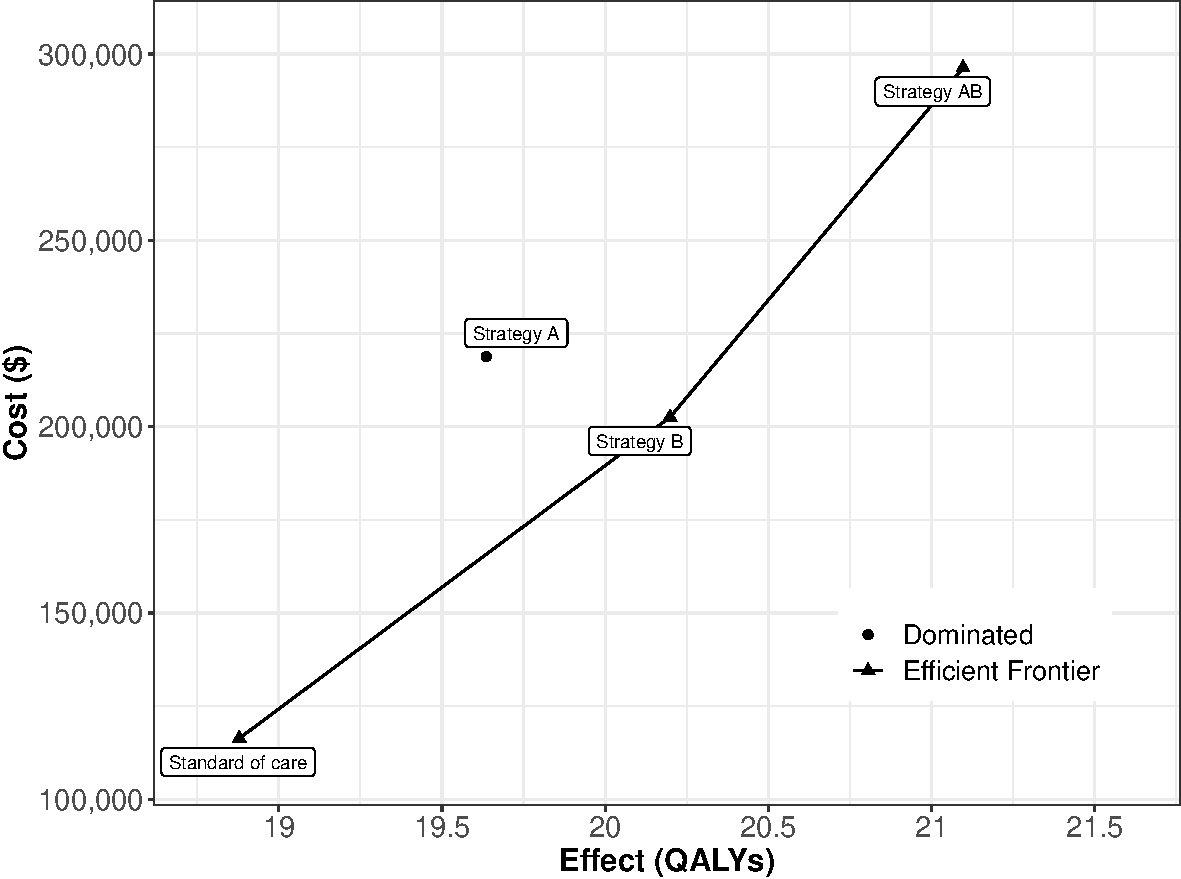
\includegraphics{figs/Sick-Sicker-CEA-AgeDep-1} 

}

\caption{Cost-effectiveness efficient frontier of all four strategies for the simulation-time-dependent Sick-Sicker model.}\label{fig:Sick-Sicker-CEA-AgeDep}
\end{figure}

\hypertarget{probabilistic-sensitivity-analysis}{%
\section{Probabilistic sensitivity analysis}\label{probabilistic-sensitivity-analysis}}

We conducted a probabilistic sensitivity analysis (PSA) to quantify the effect of model parameter uncertainty on cost-effectiveness outcomes.\textsuperscript{\protect\hyperlink{ref-Briggs2012}{24}} In a PSA, we randomly draw parameter sets from distributions that reflect the current uncertainty in model parameter estimates. The parameters' distributions and their values are described in Table \ref{tab:param-table} and more detail in the Supplementary Material. We compute model outcomes for each sampled set of parameter values (e.g., total discounted cost and QALYs) for each strategy. We follow the steps to conduct a PSA from a previously published article describing the Decision Analysis in R for technologies in Health (DARTH) coding framework.\textsuperscript{\protect\hyperlink{ref-Alarid-Escudero2019e}{13}}

To conduct the PSA of the CEA using the simulation-time-dependent Sick-Sicker cSTM, we sampled 1,000 parameter sets. For each set, we computed the total discounted costs and QALYs of each simulated strategy. Results from a PSA can be represented in various ways. For example, the joint distribution, 95\% confidence ellipse, and the expected values of the total discounted costs and QALYs for each strategy can be plotted in a cost-effectiveness (CE) scatter plot (Figure \ref{fig:CE-scatter-TimeDep}),\textsuperscript{\protect\hyperlink{ref-Briggs2002}{25}} where each of the 4,000 simulations (i.e., 1,000 combinations of total discounted expected costs and QALYs for each of the four strategies) are plotted as a point in the graph. The CE scatter plot for the CEA using the simulation-time-dependent model shows that strategy AB has the highest expected costs and QALYs. Standard of care has the lowest expected cost and QALYs. Strategy B is more effective and least costly than strategy A. And therefore, strategy A is strongly dominated by strategy B.

\begin{figure}[H]

{\centering 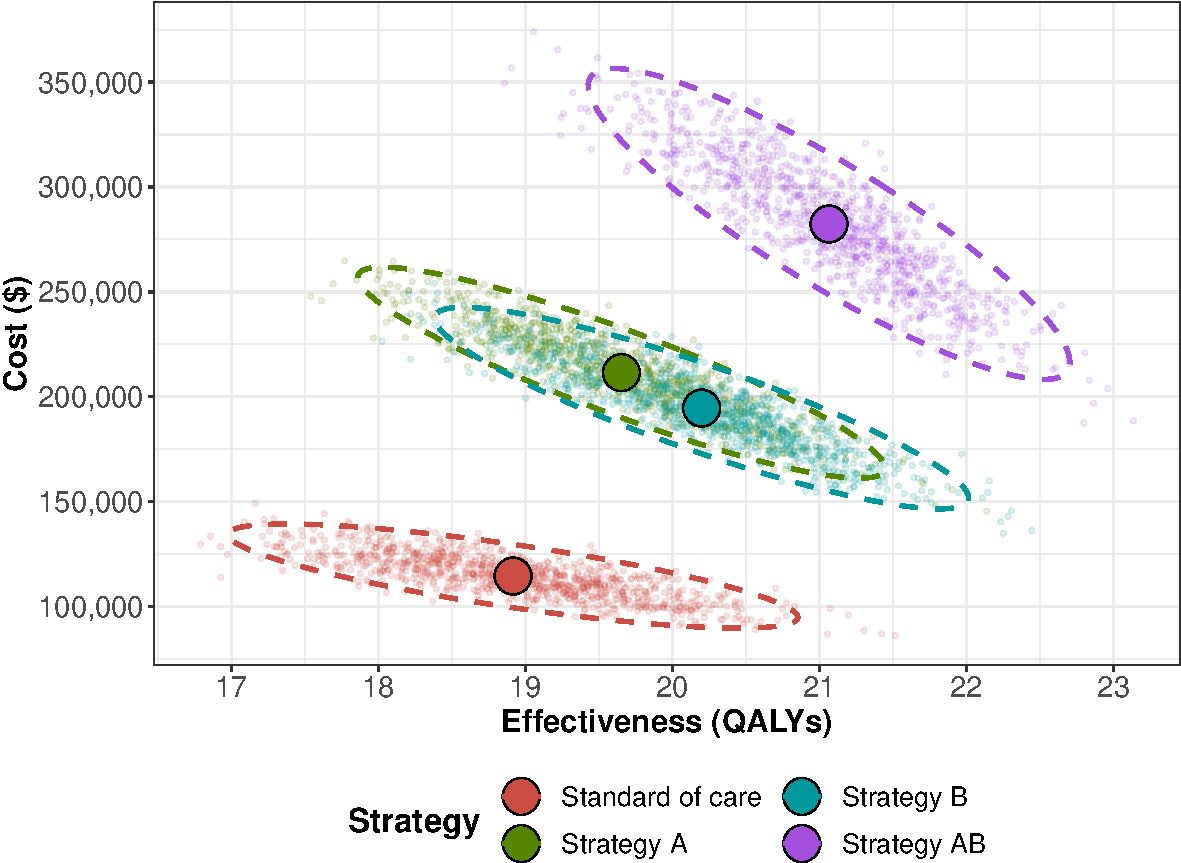
\includegraphics{figs/CE-scatter-TimeDep-1} 

}

\caption{Cost-effectiveness scatter plot.}\label{fig:CE-scatter-TimeDep}
\end{figure}

In Figure \ref{fig:CEAC-AgeDep}, we present the cost-effectiveness acceptability curves (CEACs) showing the probability that each strategy is cost-effective, and the cost-effectiveness frontier (CEAF), which shows the strategy with the highest expected net monetary benefit (NMB), over a range of willingness-to-pay (WTP) thresholds. Each strategy's NMB is computed using \(\text{NMB} = \text{QALY} \times \text{WTP} - \text{Cost}\)\textsuperscript{\protect\hyperlink{ref-Stinnett1998b}{26}} for each PSA sample. At WTP thresholds less than \$65,000 per QALY, SoC is the strategy with the highest probability of being cost-effective and the highest expected NMB. Strategy B has the highest probability of being cost-effective and the highest expected NMB for WTP thresholds greater than \$65,000 and smaller than \$105,000 per QALY. Strategy AB, has the highest expected NMB for WTP thresholds greater than or equal to \$105,000 and is the strategy with the highest probability of being cost-effective.

\begin{figure}[H]

{\centering 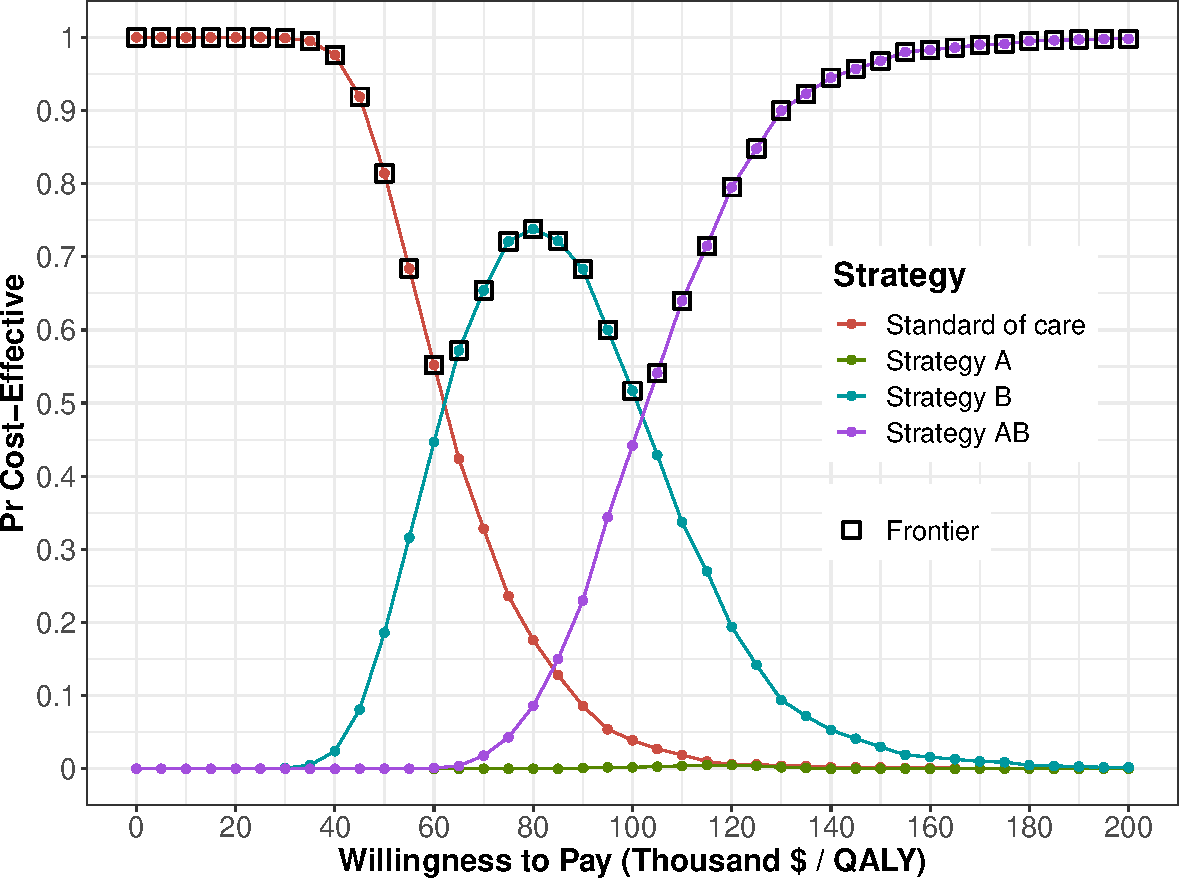
\includegraphics{figs/CEAC-AgeDep-1} 

}

\caption{Cost-effectiveness acceptability curves (CEACs) and frontier (CEAF).}\label{fig:CEAC-AgeDep}
\end{figure}

The CEAC and CEAF do not show the magnitude of the expected net benefit lost (i.e., expected loss) when the chosen strategy is not the cost-effective strategy in all the samples of the PSA. We quantify expected loss from each strategy over a range of WTP thresholds with the expected loss curves (ELCs) to complement these results (Figure \ref{fig:ELC-AgeDep}). The expected loss considers both the probability of making the wrong decision and the magnitude of the loss due to this decision, representing the foregone benefits of choosing a suboptimal strategy. The expected loss of the optimal strategy represents the lowest envelope of the ELCs because, given current information, the loss cannot be minimized further. The lower envelope also represents the expected value of perfect information (EVPI), which quantifies the value of eliminating parameter uncertainty. The strategy SoC has the lowest expected loss for WTP thresholds less than \$60,000 per QALY, strategy B has the lowest expected loss for WTP threshold greater than or equal to \$65,000 and less than \$105,000. Strategy AB has the lowest expected loss for WTP threshold greater than or equal to \$105,000 per QALY. At a WTP threshold of \$65,000 per QALY, the EVPI is highest at \$6,953. For a more detailed description of these outputs and the R code to generate them, we refer the reader to a previous publication by our group.\textsuperscript{\protect\hyperlink{ref-Alarid-Escudero2019}{27}}

\begin{figure}[H]

{\centering 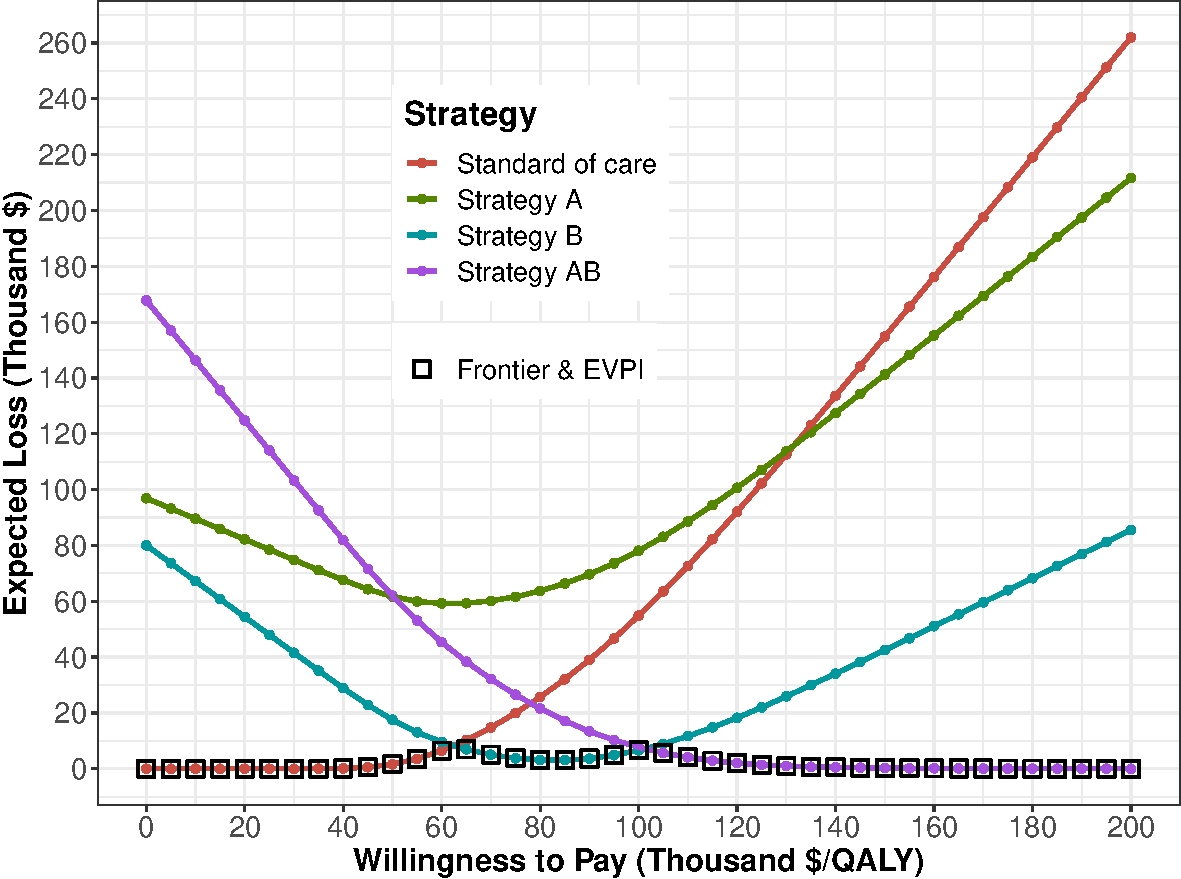
\includegraphics{figs/ELC-AgeDep-1} 

}

\caption{Expected loss curves (ELCs) and expected value of perfect information (EVPI).}\label{fig:ELC-AgeDep}
\end{figure}

\hypertarget{discussion}{%
\section{Discussion}\label{discussion}}

In this tutorial, we provided a conceptualization of time-dependent cSTMs with their mathematical description and a walk-through of their implementation for CEA in R using the Sick-Sicker example. We described two types of time-dependency: dependence on the time since the start of the simulation (simulation-time dependency) or dependence on the time spent in a health state (state-residence dependency). In addition, we illustrated how to generate various epidemiological measures from the model and how to incorporate transition rewards in CEAs.

In our example model, we implement simulation-time dependence by expanding the transition probability matrix into a transition probability array, where the third dimension captures time. However, there are alternative implementations of simulation-time dependence in cSTMs. For example, another approach would be to update the time-varying elements of the transition probability matrix \(P_t\) at each time point \(t\). That would alleviate the need for the construction of the array \texttt{a\_P}. Updating the transition matrix at each cycle can reduce computer memory requirements but at the expense of increasing the number of operations in the update of \(P_t\) at every cycle. Another approach to account for history dependence is to use a 3-dimensional transition probability matrix with dimensions for the current state, future state, and time in the current state.\textsuperscript{\protect\hyperlink{ref-Hawkins2005}{28}} However, this multidimensional matrix will have to be expanded by another dimension to incorporate age dependence by replicating the states for as many age groups considered in the model. In this tutorial, we used the third dimension as the cohort's age. We incorporated state-residence time dependency by expanding the corresponding health states on the second dimension of the 3-dimensional array to account for time spent in the current state. This approach's benefit is that we can still use the transition dynamics array to capture all states' transitions for all cycles.

The parameterization of our example model assumes all parameters are known, or at least, the characterization of their uncertainty is known (i.e., we know their distributions). However, to construct a real-world cSTM, modelers must conduct a thorough synthesis of current evidence to determine the appropriate model structure and parameter values. For example, the transition probabilities between non-death health states may be estimated in the literature as conditional on being alive or as competing risks with dying; the estimation assumptions behind parameter values should be compatible with how those parameters are used to implement model dynamics.\textsuperscript{\protect\hyperlink{ref-Briggs2012}{24}} Similarly, our PSA analysis simplifies reality by assuming that all model parameters are independent of each other. More realistically, parameters are often correlated with each other or have a rank order that should be preserved. In such cases, more complex statistical methods that simulate these correlations or rank orderings are needed.\textsuperscript{\protect\hyperlink{ref-Goldhaber-Fiebert2015}{29}} Modelers should also take care to correctly specify all model parameters for the cycle length of the model. For example, adjusting an annual mortality rate to a weekly probability requires some probability conversion.\textsuperscript{\protect\hyperlink{ref-Hunink2014}{30}}

As described in the accompanying tutorial, cSTMs are recommended when the number of states is considered ``not too large''.\textsuperscript{\protect\hyperlink{ref-Siebert2012c}{16}} This recommendation arises because as the number of states increases, it becomes more challenging to keep track of their construction. It is possible to build reasonably complex cSTMs in R as long as the size of the transition probability matrix and outputs of interest can be stored in the computer's RAM running the analysis. For example, a typical PC with 8GB of RAM can handle a transition probability array of about 1000 states and 600 time-cycle slices. However, these matrices can grow quickly, and if the required number of states gets too large and difficult to manage its coding, it becomes preferable to use a stochastic (Monte Carlo) version of the state-transition model -- often called individual-based state-transition models (iSTM) or microsimulation models -- rather than a cohort simulation model.\textsuperscript{\protect\hyperlink{ref-Siebert2012c}{16}} In an iSTM, the risks and rewards of simulated individuals need not depend only on a current health state; it may also depend on their characteristics and attributes. In addition, modelers can store health state history and other events over time for each individual to determine the risk of new events and corresponding costs and effects. Thus, we recommend thinking about the required model structure before implementing it some model structures might remain the same. An iSTM will also require additional functions to describe the dependency of transition probabilities and rewards on individuals' history. In a previous tutorial, we showed how to construct these functions for an iSTM using the Sick-Sicker example.\textsuperscript{\protect\hyperlink{ref-Krijkamp2018}{12}}

In summary, this tutorial extends our conceptualization of time-independent cSTMs to allow for time dependency. It provides a step-by-step guide to implement them in R. We hope that health decision scientists and health economists find this tutorial useful for developing their cSTMs in a more flexible, efficient, and open-source manner. Ultimately, our goal is to increase model transparency and reproducibility.

\hypertarget{acknowledgements}{%
\section{Acknowledgements}\label{acknowledgements}}

Dr Alarid-Escudero was supported by grants U01-CA199335 and U01-CA253913 from the National Cancer Institute (NCI) as part of the Cancer Intervention and Surveillance Modeling Network (CISNET), and a grant by the Gordon and Betty Moore Foundation. Miss Krijkamp was supported by the Society for Medical Decision Making (SMDM) fellowship through a grant by the Gordon and Betty Moore Foundation (GBMF7853). Dr Enns was supported by a grant from the National Institute of Allergy and Infectious Diseases of the National Institutes of Health under award no. K25AI118476. Dr.~Hunink received research funding from the American Diabetes Association, the Netherlands Organization for Health Research and Development, the German Innovation Fund, Netherlands Educational Grant (``Studie Voorschot Middelen''), and the Gordon and Betty Moore Foundation. Dr Jalal was supported by a grant from the National Institute on Drug Abuse of the National Institute of Health under award no. K01DA048985. The content is solely the responsibility of the authors and does not necessarily represent the official views of the National Institutes of Health. The funding agencies had no role in the design of the study, interpretation of results, or writing of the manuscript. The funding agreement ensured the authors' independence in designing the study, interpreting the data, writing, and publishing the report. We also want to thank the anonymous reviewers of \emph{Medical Decision Making} for their valuable suggestions and the students who took our classes where we refined these materials.

\hypertarget{references}{%
\section*{References}\label{references}}
\addcontentsline{toc}{section}{References}

\hypertarget{refs}{}
\begin{CSLReferences}{0}{0}
\leavevmode\hypertarget{ref-Suijkerbuijk2018}{}%
\CSLLeftMargin{1. }
\CSLRightInline{Suijkerbuijk AWM, Van Hoek AJ, Koopsen J, et al. {Cost-effectiveness of screening for chronic hepatitis B and C among migrant populations in a low endemic country}. \emph{PLoS ONE} 2018; 13: 1--16.}

\leavevmode\hypertarget{ref-Sathianathen2018a}{}%
\CSLLeftMargin{2. }
\CSLRightInline{Sathianathen NJ, Konety BR, Alarid-Escudero F, et al. {Cost-effectiveness Analysis of Active Surveillance Strategies for Men with Low-risk Prostate Cancer}. \emph{European Urology}; 75: 910--917, \url{https://linkinghub.elsevier.com/retrieve/pii/S0302283818308534} (2019).}

\leavevmode\hypertarget{ref-Lu2018b}{}%
\CSLLeftMargin{3. }
\CSLRightInline{Lu S, Yu Y, Fu S, et al. {Cost-effectiveness of ALK testing and first-line crizotinib therapy for non-small-cell lung cancer in China}. \emph{PLoS ONE} 2018; 13: 1--12.}

\leavevmode\hypertarget{ref-Djatche2018}{}%
\CSLLeftMargin{4. }
\CSLRightInline{Djatche LM, Varga S, Lieberthal RD. {Cost-Effectiveness of Aspirin Adherence for Secondary Prevention of Cardiovascular Events}. \emph{PharmacoEconomics - Open}; 2: 371--380, \url{https://doi.org/10.1007/s41669-018-0075-2} (2018).}

\leavevmode\hypertarget{ref-Pershing2014}{}%
\CSLLeftMargin{5. }
\CSLRightInline{Pershing S, Enns EA, Matesic B, et al. {Cost-Effectiveness of Treatment of Diabetic Macular Edema}. \emph{Annals of Internal Medicine} 2014; 160: 18--29.}

\leavevmode\hypertarget{ref-Smith-Spangler2010}{}%
\CSLLeftMargin{6. }
\CSLRightInline{Smith-Spangler CM, Juusola JL, Enns EA, et al. {Population Strategies to Decrease Sodium Intake and the Burden of Cardiovascular Disease: A Cost-Effectiveness Analysis}. \emph{Annals of Internal Medicine}; 152: 481--487, \url{http://annals.org/article.aspx?articleid=745729} (2010).}

\leavevmode\hypertarget{ref-Alarid-Escudero2021a}{}%
\CSLLeftMargin{7. }
\CSLRightInline{Alarid-Escudero F, Krijkamp E, Enns EA, et al. {An Introductory Tutorial to Cohort State-Transition Models in R}. 2021.}

\leavevmode\hypertarget{ref-Snowsill2019}{}%
\CSLLeftMargin{8. }
\CSLRightInline{Snowsill T. {A New Method for Model-Based Health Economic Evaluation Utilizing and Extending Moment-Generating Functions}. \emph{Medical Decision Making}; 39: 523--539, \url{http://journals.sagepub.com/doi/10.1177/0272989X19860119} (2019).}

\leavevmode\hypertarget{ref-Krijkamp2019}{}%
\CSLLeftMargin{9. }
\CSLRightInline{Krijkamp EM, Alarid-Escudero F, Enns E, et al. {A Multidimensional Array Representation of State-Transition Model Dynamics}. \emph{Medical Decision Making} 2019; In Press.}

\leavevmode\hypertarget{ref-Jalal2017b}{}%
\CSLLeftMargin{10. }
\CSLRightInline{Jalal H, Pechlivanoglou P, Krijkamp E, et al. {An Overview of R in Health Decision Sciences}. \emph{Medical Decision Making}; 37: 735--746, \url{http://journals.sagepub.com/doi/10.1177/0272989X16686559} (2017).}

\leavevmode\hypertarget{ref-Enns2015e}{}%
\CSLLeftMargin{11. }
\CSLRightInline{Enns EA, Cipriano LE, Simons CT, et al. {Identifying Best-Fitting Inputs in Health-Economic Model Calibration: A Pareto Frontier Approach}. \emph{Medical Decision Making}; 35: 170--182, \url{http://www.ncbi.nlm.nih.gov/pubmed/24799456} (2015).}

\leavevmode\hypertarget{ref-Krijkamp2018}{}%
\CSLLeftMargin{12. }
\CSLRightInline{Krijkamp EM, Alarid-Escudero F, Enns EA, et al. {Microsimulation Modeling for Health Decision Sciences Using R: A Tutorial}. \emph{Medical Decision Making}; 38: 400--422, \url{http://journals.sagepub.com/doi/10.1177/0272989X18754513} (2018).}

\leavevmode\hypertarget{ref-Alarid-Escudero2019e}{}%
\CSLLeftMargin{13. }
\CSLRightInline{Alarid-Escudero F, Krijkamp E, Pechlivanoglou P, et al. {A Need for Change! A Coding Framework for Improving Transparency in Decision Modeling}. \emph{PharmacoEconomics}; 37: 1329--1339, \url{https://doi.org/10.1007/s40273-019-00837-x} (2019).}

\leavevmode\hypertarget{ref-Arias2017}{}%
\CSLLeftMargin{14. }
\CSLRightInline{Arias E, Heron M, Xu J. {United States Life Tables, 2014}. \emph{National Vital Statistics Reports}; 66: 63, \url{https://www.cdc.gov/nchs/data/nvsr/nvsr66/nvsr66\%7B/_\%7D04.pdf} (2017).}

\leavevmode\hypertarget{ref-Diaby2014}{}%
\CSLLeftMargin{15. }
\CSLRightInline{Diaby V, Adunlin G, Montero AJ. {Survival modeling for the estimation of transition probabilities in model-based economic evaluations in the absence of individual patient data: A tutorial}. \emph{PharmacoEconomics} 2014; 32: 101--108.}

\leavevmode\hypertarget{ref-Siebert2012c}{}%
\CSLLeftMargin{16. }
\CSLRightInline{Siebert U, Alagoz O, Bayoumi AM, et al. {State-Transition Modeling: A Report of the ISPOR-SMDM Modeling Good Research Practices Task Force-3}. \emph{Medical Decision Making}; 32: 690--700, \url{http://mdm.sagepub.com/cgi/doi/10.1177/0272989X12455463} (2012).}

\leavevmode\hypertarget{ref-Lee2003a}{}%
\CSLLeftMargin{17. }
\CSLRightInline{Lee ET, Wang JW. \emph{{Statistical methods for Survival Data Analysis}}. 3rd ed. Hoboken, NJ: Wiley, 2003.}

\leavevmode\hypertarget{ref-Klein2003}{}%
\CSLLeftMargin{18. }
\CSLRightInline{Klein JP, Moeschberger ML. \emph{{Survival Analysis: Techniques for Censored and Truncated Data}}. 2nd ed. Springer-Verlag, \url{http://www.springer.com/statistics/life+sciences,+medicine+\%7B/\&\%7D+health/book/978-0-387-95399-1} (2003).}

\leavevmode\hypertarget{ref-Rothman2008h}{}%
\CSLLeftMargin{19. }
\CSLRightInline{Rothman KJ, Greenland S, Lash TL. \emph{{Modern Epidemiology}}. 3rd ed. Lippincott Williams {\&} Wilkins, 2008.}

\leavevmode\hypertarget{ref-Keiding1991}{}%
\CSLLeftMargin{20. }
\CSLRightInline{Keiding N. {Age-Specific Incidence and Prevalence: A Statistical Perspective}. \emph{Journal of the Royal Statistical Society Series A (Statistics in Society)} 1991; 154: 371--412.}

\leavevmode\hypertarget{ref-Elbasha2016}{}%
\CSLLeftMargin{21. }
\CSLRightInline{Elbasha EH, Chhatwal J. {Theoretical foundations and practical applications of within-cycle correction methods}. \emph{Medical Decision Making} 2016; 36: 115--131.}

\leavevmode\hypertarget{ref-Elbasha2016a}{}%
\CSLLeftMargin{22. }
\CSLRightInline{Elbasha EH, Chhatwal J. {Myths and misconceptions of within-cycle correction: a guide for modelers and decision makers}. \emph{PharmacoEconomics} 2016; 34: 13--22.}

\leavevmode\hypertarget{ref-Alarid-Escudero2021}{}%
\CSLLeftMargin{23. }
\CSLRightInline{Alarid-Escudero F, Knowlton G, Easterly CA, et al. Decision analytic modeling package (dampack), \url{https://cran.r-project.org/web/packages/dampack/\%20https://github.com/DARTH-git/dampack} (2021).}

\leavevmode\hypertarget{ref-Briggs2012}{}%
\CSLLeftMargin{24. }
\CSLRightInline{Briggs AH, Weinstein MC, Fenwick EAL, et al. {Model Parameter Estimation and Uncertainty Analysis: A Report of the ISPOR-SMDM Modeling Good Research Practices Task Force Working Group-6.} \emph{Medical Decision Making} 2012; 32: 722--732.}

\leavevmode\hypertarget{ref-Briggs2002}{}%
\CSLLeftMargin{25. }
\CSLRightInline{Briggs AH, Goeree R, Blackhouse G, et al. {Probabilistic Analysis of Cost-Effectiveness Models: Choosing between Treatment Strategies for Gastroesophageal Reflux Disease}. \emph{Medical Decision Making}; 22: 290--308, \url{http://mdm.sagepub.com/cgi/doi/10.1177/027298902400448867} (2002).}

\leavevmode\hypertarget{ref-Stinnett1998b}{}%
\CSLLeftMargin{26. }
\CSLRightInline{Stinnett AA, Mullahy J. {Net Health Benefits: A New Framework for the Analysis of Uncertainty in Cost-Effectiveness Analysis}. \emph{Medical Decision Making}; 18: S68--S80, \url{http://mdm.sagepub.com/cgi/doi/10.1177/0272989X9801800209} (1998).}

\leavevmode\hypertarget{ref-Alarid-Escudero2019}{}%
\CSLLeftMargin{27. }
\CSLRightInline{Alarid-Escudero F, Enns EA, Kuntz KM, et al. {"Time Traveling Is Just Too Dangerous" But Some Methods Are Worth Revisiting: The Advantages of Expected Loss Curves Over Cost-Effectiveness Acceptability Curves and Frontier}. \emph{Value in Health} 2019; 22: 611--618.}

\leavevmode\hypertarget{ref-Hawkins2005}{}%
\CSLLeftMargin{28. }
\CSLRightInline{Hawkins N, Sculpher M, Epstein D. {Cost-effectiveness analysis of treatments for chronic disease: Using R to incorporate time dependency of treatment response.} \emph{Medical Decision Making}; 25: 511--9, \url{http://www.ncbi.nlm.nih.gov/pubmed/16160207} (2005).}

\leavevmode\hypertarget{ref-Goldhaber-Fiebert2015}{}%
\CSLLeftMargin{29. }
\CSLRightInline{Goldhaber-Fiebert JD, Jalal HJ. {Some Health States Are Better Than Others: Using Health State Rank Order to Improve Probabilistic Analyses}. \emph{Medical Decision Making}; 36: 927--940, \url{http://mdm.sagepub.com/cgi/doi/10.1177/0272989X15605091} (2015).}

\leavevmode\hypertarget{ref-Hunink2014}{}%
\CSLLeftMargin{30. }
\CSLRightInline{Hunink MGGM, Weinstein MC, Wittenberg E, et al. \emph{{Decision Making in Health and Medicine}}. 2nd ed. Cambridge: Cambridge University Press, \url{http://ebooks.cambridge.org/ref/id/CBO9781139506779} (2014).}

\end{CSLReferences}

\end{document}
